
% Default to the notebook output style

    


% Inherit from the specified cell style.




    
\documentclass[11pt]{article}

    
    
    \usepackage[T1]{fontenc}
    % Nicer default font (+ math font) than Computer Modern for most use cases
    \usepackage{mathpazo}

    % Basic figure setup, for now with no caption control since it's done
    % automatically by Pandoc (which extracts ![](path) syntax from Markdown).
    \usepackage{graphicx}
    % We will generate all images so they have a width \maxwidth. This means
    % that they will get their normal width if they fit onto the page, but
    % are scaled down if they would overflow the margins.
    \makeatletter
    \def\maxwidth{\ifdim\Gin@nat@width>\linewidth\linewidth
    \else\Gin@nat@width\fi}
    \makeatother
    \let\Oldincludegraphics\includegraphics
    % Set max figure width to be 80% of text width, for now hardcoded.
    \renewcommand{\includegraphics}[1]{\Oldincludegraphics[width=.8\maxwidth]{#1}}
    % Ensure that by default, figures have no caption (until we provide a
    % proper Figure object with a Caption API and a way to capture that
    % in the conversion process - todo).
    \usepackage{caption}
    \DeclareCaptionLabelFormat{nolabel}{}
    \captionsetup{labelformat=nolabel}

    \usepackage{adjustbox} % Used to constrain images to a maximum size 
    \usepackage{xcolor} % Allow colors to be defined
    \usepackage{enumerate} % Needed for markdown enumerations to work
    \usepackage{geometry} % Used to adjust the document margins
    \usepackage{amsmath} % Equations
    \usepackage{amssymb} % Equations
    \usepackage{textcomp} % defines textquotesingle
    % Hack from http://tex.stackexchange.com/a/47451/13684:
    \AtBeginDocument{%
        \def\PYZsq{\textquotesingle}% Upright quotes in Pygmentized code
    }
    \usepackage{upquote} % Upright quotes for verbatim code
    \usepackage{eurosym} % defines \euro
    \usepackage[mathletters]{ucs} % Extended unicode (utf-8) support
    \usepackage[utf8x]{inputenc} % Allow utf-8 characters in the tex document
    \usepackage{fancyvrb} % verbatim replacement that allows latex
    \usepackage{grffile} % extends the file name processing of package graphics 
                         % to support a larger range 
    % The hyperref package gives us a pdf with properly built
    % internal navigation ('pdf bookmarks' for the table of contents,
    % internal cross-reference links, web links for URLs, etc.)
    \usepackage{hyperref}
    \usepackage{longtable} % longtable support required by pandoc >1.10
    \usepackage{booktabs}  % table support for pandoc > 1.12.2
    \usepackage[inline]{enumitem} % IRkernel/repr support (it uses the enumerate* environment)
    \usepackage[normalem]{ulem} % ulem is needed to support strikethroughs (\sout)
                                % normalem makes italics be italics, not underlines
    

    
    
    % Colors for the hyperref package
    \definecolor{urlcolor}{rgb}{0,.145,.698}
    \definecolor{linkcolor}{rgb}{.71,0.21,0.01}
    \definecolor{citecolor}{rgb}{.12,.54,.11}

    % ANSI colors
    \definecolor{ansi-black}{HTML}{3E424D}
    \definecolor{ansi-black-intense}{HTML}{282C36}
    \definecolor{ansi-red}{HTML}{E75C58}
    \definecolor{ansi-red-intense}{HTML}{B22B31}
    \definecolor{ansi-green}{HTML}{00A250}
    \definecolor{ansi-green-intense}{HTML}{007427}
    \definecolor{ansi-yellow}{HTML}{DDB62B}
    \definecolor{ansi-yellow-intense}{HTML}{B27D12}
    \definecolor{ansi-blue}{HTML}{208FFB}
    \definecolor{ansi-blue-intense}{HTML}{0065CA}
    \definecolor{ansi-magenta}{HTML}{D160C4}
    \definecolor{ansi-magenta-intense}{HTML}{A03196}
    \definecolor{ansi-cyan}{HTML}{60C6C8}
    \definecolor{ansi-cyan-intense}{HTML}{258F8F}
    \definecolor{ansi-white}{HTML}{C5C1B4}
    \definecolor{ansi-white-intense}{HTML}{A1A6B2}

    % commands and environments needed by pandoc snippets
    % extracted from the output of `pandoc -s`
    \providecommand{\tightlist}{%
      \setlength{\itemsep}{0pt}\setlength{\parskip}{0pt}}
    \DefineVerbatimEnvironment{Highlighting}{Verbatim}{commandchars=\\\{\}}
    % Add ',fontsize=\small' for more characters per line
    \newenvironment{Shaded}{}{}
    \newcommand{\KeywordTok}[1]{\textcolor[rgb]{0.00,0.44,0.13}{\textbf{{#1}}}}
    \newcommand{\DataTypeTok}[1]{\textcolor[rgb]{0.56,0.13,0.00}{{#1}}}
    \newcommand{\DecValTok}[1]{\textcolor[rgb]{0.25,0.63,0.44}{{#1}}}
    \newcommand{\BaseNTok}[1]{\textcolor[rgb]{0.25,0.63,0.44}{{#1}}}
    \newcommand{\FloatTok}[1]{\textcolor[rgb]{0.25,0.63,0.44}{{#1}}}
    \newcommand{\CharTok}[1]{\textcolor[rgb]{0.25,0.44,0.63}{{#1}}}
    \newcommand{\StringTok}[1]{\textcolor[rgb]{0.25,0.44,0.63}{{#1}}}
    \newcommand{\CommentTok}[1]{\textcolor[rgb]{0.38,0.63,0.69}{\textit{{#1}}}}
    \newcommand{\OtherTok}[1]{\textcolor[rgb]{0.00,0.44,0.13}{{#1}}}
    \newcommand{\AlertTok}[1]{\textcolor[rgb]{1.00,0.00,0.00}{\textbf{{#1}}}}
    \newcommand{\FunctionTok}[1]{\textcolor[rgb]{0.02,0.16,0.49}{{#1}}}
    \newcommand{\RegionMarkerTok}[1]{{#1}}
    \newcommand{\ErrorTok}[1]{\textcolor[rgb]{1.00,0.00,0.00}{\textbf{{#1}}}}
    \newcommand{\NormalTok}[1]{{#1}}
    
    % Additional commands for more recent versions of Pandoc
    \newcommand{\ConstantTok}[1]{\textcolor[rgb]{0.53,0.00,0.00}{{#1}}}
    \newcommand{\SpecialCharTok}[1]{\textcolor[rgb]{0.25,0.44,0.63}{{#1}}}
    \newcommand{\VerbatimStringTok}[1]{\textcolor[rgb]{0.25,0.44,0.63}{{#1}}}
    \newcommand{\SpecialStringTok}[1]{\textcolor[rgb]{0.73,0.40,0.53}{{#1}}}
    \newcommand{\ImportTok}[1]{{#1}}
    \newcommand{\DocumentationTok}[1]{\textcolor[rgb]{0.73,0.13,0.13}{\textit{{#1}}}}
    \newcommand{\AnnotationTok}[1]{\textcolor[rgb]{0.38,0.63,0.69}{\textbf{\textit{{#1}}}}}
    \newcommand{\CommentVarTok}[1]{\textcolor[rgb]{0.38,0.63,0.69}{\textbf{\textit{{#1}}}}}
    \newcommand{\VariableTok}[1]{\textcolor[rgb]{0.10,0.09,0.49}{{#1}}}
    \newcommand{\ControlFlowTok}[1]{\textcolor[rgb]{0.00,0.44,0.13}{\textbf{{#1}}}}
    \newcommand{\OperatorTok}[1]{\textcolor[rgb]{0.40,0.40,0.40}{{#1}}}
    \newcommand{\BuiltInTok}[1]{{#1}}
    \newcommand{\ExtensionTok}[1]{{#1}}
    \newcommand{\PreprocessorTok}[1]{\textcolor[rgb]{0.74,0.48,0.00}{{#1}}}
    \newcommand{\AttributeTok}[1]{\textcolor[rgb]{0.49,0.56,0.16}{{#1}}}
    \newcommand{\InformationTok}[1]{\textcolor[rgb]{0.38,0.63,0.69}{\textbf{\textit{{#1}}}}}
    \newcommand{\WarningTok}[1]{\textcolor[rgb]{0.38,0.63,0.69}{\textbf{\textit{{#1}}}}}
    
    
    % Define a nice break command that doesn't care if a line doesn't already
    % exist.
    \def\br{\hspace*{\fill} \\* }
    % Math Jax compatability definitions
    \def\gt{>}
    \def\lt{<}
    % Document parameters
    \title{Presentation}
    
    
    

    % Pygments definitions
    
\makeatletter
\def\PY@reset{\let\PY@it=\relax \let\PY@bf=\relax%
    \let\PY@ul=\relax \let\PY@tc=\relax%
    \let\PY@bc=\relax \let\PY@ff=\relax}
\def\PY@tok#1{\csname PY@tok@#1\endcsname}
\def\PY@toks#1+{\ifx\relax#1\empty\else%
    \PY@tok{#1}\expandafter\PY@toks\fi}
\def\PY@do#1{\PY@bc{\PY@tc{\PY@ul{%
    \PY@it{\PY@bf{\PY@ff{#1}}}}}}}
\def\PY#1#2{\PY@reset\PY@toks#1+\relax+\PY@do{#2}}

\expandafter\def\csname PY@tok@w\endcsname{\def\PY@tc##1{\textcolor[rgb]{0.73,0.73,0.73}{##1}}}
\expandafter\def\csname PY@tok@c\endcsname{\let\PY@it=\textit\def\PY@tc##1{\textcolor[rgb]{0.25,0.50,0.50}{##1}}}
\expandafter\def\csname PY@tok@cp\endcsname{\def\PY@tc##1{\textcolor[rgb]{0.74,0.48,0.00}{##1}}}
\expandafter\def\csname PY@tok@k\endcsname{\let\PY@bf=\textbf\def\PY@tc##1{\textcolor[rgb]{0.00,0.50,0.00}{##1}}}
\expandafter\def\csname PY@tok@kp\endcsname{\def\PY@tc##1{\textcolor[rgb]{0.00,0.50,0.00}{##1}}}
\expandafter\def\csname PY@tok@kt\endcsname{\def\PY@tc##1{\textcolor[rgb]{0.69,0.00,0.25}{##1}}}
\expandafter\def\csname PY@tok@o\endcsname{\def\PY@tc##1{\textcolor[rgb]{0.40,0.40,0.40}{##1}}}
\expandafter\def\csname PY@tok@ow\endcsname{\let\PY@bf=\textbf\def\PY@tc##1{\textcolor[rgb]{0.67,0.13,1.00}{##1}}}
\expandafter\def\csname PY@tok@nb\endcsname{\def\PY@tc##1{\textcolor[rgb]{0.00,0.50,0.00}{##1}}}
\expandafter\def\csname PY@tok@nf\endcsname{\def\PY@tc##1{\textcolor[rgb]{0.00,0.00,1.00}{##1}}}
\expandafter\def\csname PY@tok@nc\endcsname{\let\PY@bf=\textbf\def\PY@tc##1{\textcolor[rgb]{0.00,0.00,1.00}{##1}}}
\expandafter\def\csname PY@tok@nn\endcsname{\let\PY@bf=\textbf\def\PY@tc##1{\textcolor[rgb]{0.00,0.00,1.00}{##1}}}
\expandafter\def\csname PY@tok@ne\endcsname{\let\PY@bf=\textbf\def\PY@tc##1{\textcolor[rgb]{0.82,0.25,0.23}{##1}}}
\expandafter\def\csname PY@tok@nv\endcsname{\def\PY@tc##1{\textcolor[rgb]{0.10,0.09,0.49}{##1}}}
\expandafter\def\csname PY@tok@no\endcsname{\def\PY@tc##1{\textcolor[rgb]{0.53,0.00,0.00}{##1}}}
\expandafter\def\csname PY@tok@nl\endcsname{\def\PY@tc##1{\textcolor[rgb]{0.63,0.63,0.00}{##1}}}
\expandafter\def\csname PY@tok@ni\endcsname{\let\PY@bf=\textbf\def\PY@tc##1{\textcolor[rgb]{0.60,0.60,0.60}{##1}}}
\expandafter\def\csname PY@tok@na\endcsname{\def\PY@tc##1{\textcolor[rgb]{0.49,0.56,0.16}{##1}}}
\expandafter\def\csname PY@tok@nt\endcsname{\let\PY@bf=\textbf\def\PY@tc##1{\textcolor[rgb]{0.00,0.50,0.00}{##1}}}
\expandafter\def\csname PY@tok@nd\endcsname{\def\PY@tc##1{\textcolor[rgb]{0.67,0.13,1.00}{##1}}}
\expandafter\def\csname PY@tok@s\endcsname{\def\PY@tc##1{\textcolor[rgb]{0.73,0.13,0.13}{##1}}}
\expandafter\def\csname PY@tok@sd\endcsname{\let\PY@it=\textit\def\PY@tc##1{\textcolor[rgb]{0.73,0.13,0.13}{##1}}}
\expandafter\def\csname PY@tok@si\endcsname{\let\PY@bf=\textbf\def\PY@tc##1{\textcolor[rgb]{0.73,0.40,0.53}{##1}}}
\expandafter\def\csname PY@tok@se\endcsname{\let\PY@bf=\textbf\def\PY@tc##1{\textcolor[rgb]{0.73,0.40,0.13}{##1}}}
\expandafter\def\csname PY@tok@sr\endcsname{\def\PY@tc##1{\textcolor[rgb]{0.73,0.40,0.53}{##1}}}
\expandafter\def\csname PY@tok@ss\endcsname{\def\PY@tc##1{\textcolor[rgb]{0.10,0.09,0.49}{##1}}}
\expandafter\def\csname PY@tok@sx\endcsname{\def\PY@tc##1{\textcolor[rgb]{0.00,0.50,0.00}{##1}}}
\expandafter\def\csname PY@tok@m\endcsname{\def\PY@tc##1{\textcolor[rgb]{0.40,0.40,0.40}{##1}}}
\expandafter\def\csname PY@tok@gh\endcsname{\let\PY@bf=\textbf\def\PY@tc##1{\textcolor[rgb]{0.00,0.00,0.50}{##1}}}
\expandafter\def\csname PY@tok@gu\endcsname{\let\PY@bf=\textbf\def\PY@tc##1{\textcolor[rgb]{0.50,0.00,0.50}{##1}}}
\expandafter\def\csname PY@tok@gd\endcsname{\def\PY@tc##1{\textcolor[rgb]{0.63,0.00,0.00}{##1}}}
\expandafter\def\csname PY@tok@gi\endcsname{\def\PY@tc##1{\textcolor[rgb]{0.00,0.63,0.00}{##1}}}
\expandafter\def\csname PY@tok@gr\endcsname{\def\PY@tc##1{\textcolor[rgb]{1.00,0.00,0.00}{##1}}}
\expandafter\def\csname PY@tok@ge\endcsname{\let\PY@it=\textit}
\expandafter\def\csname PY@tok@gs\endcsname{\let\PY@bf=\textbf}
\expandafter\def\csname PY@tok@gp\endcsname{\let\PY@bf=\textbf\def\PY@tc##1{\textcolor[rgb]{0.00,0.00,0.50}{##1}}}
\expandafter\def\csname PY@tok@go\endcsname{\def\PY@tc##1{\textcolor[rgb]{0.53,0.53,0.53}{##1}}}
\expandafter\def\csname PY@tok@gt\endcsname{\def\PY@tc##1{\textcolor[rgb]{0.00,0.27,0.87}{##1}}}
\expandafter\def\csname PY@tok@err\endcsname{\def\PY@bc##1{\setlength{\fboxsep}{0pt}\fcolorbox[rgb]{1.00,0.00,0.00}{1,1,1}{\strut ##1}}}
\expandafter\def\csname PY@tok@kc\endcsname{\let\PY@bf=\textbf\def\PY@tc##1{\textcolor[rgb]{0.00,0.50,0.00}{##1}}}
\expandafter\def\csname PY@tok@kd\endcsname{\let\PY@bf=\textbf\def\PY@tc##1{\textcolor[rgb]{0.00,0.50,0.00}{##1}}}
\expandafter\def\csname PY@tok@kn\endcsname{\let\PY@bf=\textbf\def\PY@tc##1{\textcolor[rgb]{0.00,0.50,0.00}{##1}}}
\expandafter\def\csname PY@tok@kr\endcsname{\let\PY@bf=\textbf\def\PY@tc##1{\textcolor[rgb]{0.00,0.50,0.00}{##1}}}
\expandafter\def\csname PY@tok@bp\endcsname{\def\PY@tc##1{\textcolor[rgb]{0.00,0.50,0.00}{##1}}}
\expandafter\def\csname PY@tok@fm\endcsname{\def\PY@tc##1{\textcolor[rgb]{0.00,0.00,1.00}{##1}}}
\expandafter\def\csname PY@tok@vc\endcsname{\def\PY@tc##1{\textcolor[rgb]{0.10,0.09,0.49}{##1}}}
\expandafter\def\csname PY@tok@vg\endcsname{\def\PY@tc##1{\textcolor[rgb]{0.10,0.09,0.49}{##1}}}
\expandafter\def\csname PY@tok@vi\endcsname{\def\PY@tc##1{\textcolor[rgb]{0.10,0.09,0.49}{##1}}}
\expandafter\def\csname PY@tok@vm\endcsname{\def\PY@tc##1{\textcolor[rgb]{0.10,0.09,0.49}{##1}}}
\expandafter\def\csname PY@tok@sa\endcsname{\def\PY@tc##1{\textcolor[rgb]{0.73,0.13,0.13}{##1}}}
\expandafter\def\csname PY@tok@sb\endcsname{\def\PY@tc##1{\textcolor[rgb]{0.73,0.13,0.13}{##1}}}
\expandafter\def\csname PY@tok@sc\endcsname{\def\PY@tc##1{\textcolor[rgb]{0.73,0.13,0.13}{##1}}}
\expandafter\def\csname PY@tok@dl\endcsname{\def\PY@tc##1{\textcolor[rgb]{0.73,0.13,0.13}{##1}}}
\expandafter\def\csname PY@tok@s2\endcsname{\def\PY@tc##1{\textcolor[rgb]{0.73,0.13,0.13}{##1}}}
\expandafter\def\csname PY@tok@sh\endcsname{\def\PY@tc##1{\textcolor[rgb]{0.73,0.13,0.13}{##1}}}
\expandafter\def\csname PY@tok@s1\endcsname{\def\PY@tc##1{\textcolor[rgb]{0.73,0.13,0.13}{##1}}}
\expandafter\def\csname PY@tok@mb\endcsname{\def\PY@tc##1{\textcolor[rgb]{0.40,0.40,0.40}{##1}}}
\expandafter\def\csname PY@tok@mf\endcsname{\def\PY@tc##1{\textcolor[rgb]{0.40,0.40,0.40}{##1}}}
\expandafter\def\csname PY@tok@mh\endcsname{\def\PY@tc##1{\textcolor[rgb]{0.40,0.40,0.40}{##1}}}
\expandafter\def\csname PY@tok@mi\endcsname{\def\PY@tc##1{\textcolor[rgb]{0.40,0.40,0.40}{##1}}}
\expandafter\def\csname PY@tok@il\endcsname{\def\PY@tc##1{\textcolor[rgb]{0.40,0.40,0.40}{##1}}}
\expandafter\def\csname PY@tok@mo\endcsname{\def\PY@tc##1{\textcolor[rgb]{0.40,0.40,0.40}{##1}}}
\expandafter\def\csname PY@tok@ch\endcsname{\let\PY@it=\textit\def\PY@tc##1{\textcolor[rgb]{0.25,0.50,0.50}{##1}}}
\expandafter\def\csname PY@tok@cm\endcsname{\let\PY@it=\textit\def\PY@tc##1{\textcolor[rgb]{0.25,0.50,0.50}{##1}}}
\expandafter\def\csname PY@tok@cpf\endcsname{\let\PY@it=\textit\def\PY@tc##1{\textcolor[rgb]{0.25,0.50,0.50}{##1}}}
\expandafter\def\csname PY@tok@c1\endcsname{\let\PY@it=\textit\def\PY@tc##1{\textcolor[rgb]{0.25,0.50,0.50}{##1}}}
\expandafter\def\csname PY@tok@cs\endcsname{\let\PY@it=\textit\def\PY@tc##1{\textcolor[rgb]{0.25,0.50,0.50}{##1}}}

\def\PYZbs{\char`\\}
\def\PYZus{\char`\_}
\def\PYZob{\char`\{}
\def\PYZcb{\char`\}}
\def\PYZca{\char`\^}
\def\PYZam{\char`\&}
\def\PYZlt{\char`\<}
\def\PYZgt{\char`\>}
\def\PYZsh{\char`\#}
\def\PYZpc{\char`\%}
\def\PYZdl{\char`\$}
\def\PYZhy{\char`\-}
\def\PYZsq{\char`\'}
\def\PYZdq{\char`\"}
\def\PYZti{\char`\~}
% for compatibility with earlier versions
\def\PYZat{@}
\def\PYZlb{[}
\def\PYZrb{]}
\makeatother


    % Exact colors from NB
    \definecolor{incolor}{rgb}{0.0, 0.0, 0.5}
    \definecolor{outcolor}{rgb}{0.545, 0.0, 0.0}



    
    % Prevent overflowing lines due to hard-to-break entities
    \sloppy 
    % Setup hyperref package
    \hypersetup{
      breaklinks=true,  % so long urls are correctly broken across lines
      colorlinks=true,
      urlcolor=urlcolor,
      linkcolor=linkcolor,
      citecolor=citecolor,
      }
    % Slightly bigger margins than the latex defaults
    
    \geometry{verbose,tmargin=1in,bmargin=1in,lmargin=1in,rmargin=1in}
    
    

    \begin{document}
    
    
    \maketitle
    
    

    
    Python Libraries for GIS and Jupyter Notebook as a Mapping Application

WA Women in GIS and Technology - Wed March 6, 2019

Christy Heaton

    About me

    \begin{figure}
\centering

\includegraphics{img/FS_bio.PNG}
\caption{title}
\end{figure}

    \begin{figure}
\centering
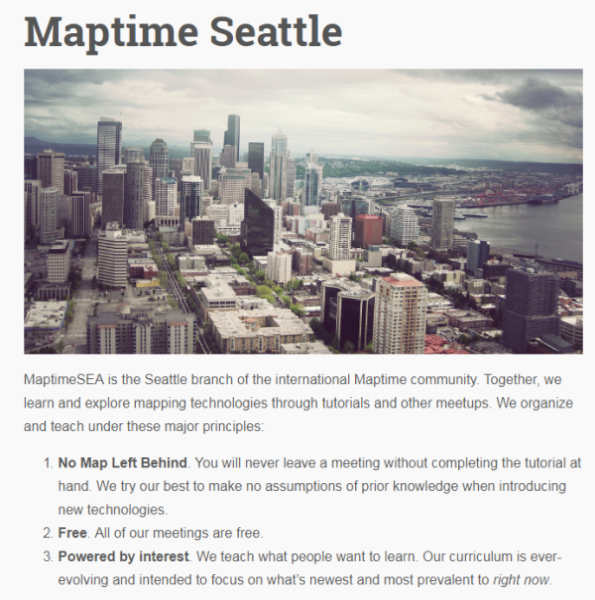
\includegraphics{img/maptimeseattle_website.PNG}
\caption{title}
\end{figure}

Find us on \href{https://www.meetup.com/MaptimeSEA}{Meetup!}

    \hypertarget{outline}{%
\section{Outline}\label{outline}}

    \hypertarget{open-source-vs.-proprietary}{%
\subsubsection{Open Source
vs.~Proprietary}\label{open-source-vs.-proprietary}}

    \hypertarget{python}{%
\subsubsection{Python}\label{python}}

    \hypertarget{jupyter-notebook}{%
\subsubsection{Jupyter Notebook}\label{jupyter-notebook}}

    \hypertarget{fun-example}{%
\subsubsection{Fun Example}\label{fun-example}}

    \hypertarget{open-source-vs.-proprietary}{%
\section{\texorpdfstring{\href{https://opensource.com/resources/what-open-source}{Open
Source
vs.~Proprietary}}{Open Source vs.~Proprietary}}\label{open-source-vs.-proprietary}}

    \hypertarget{python}{%
\section{\texorpdfstring{\href{https://www.python.org/about/}{Python}}{Python}}\label{python}}

    \hypertarget{jupyter-notebook}{%
\section{\texorpdfstring{\href{https://jupyter.org/}{Jupyter
Notebook}}{Jupyter Notebook}}\label{jupyter-notebook}}

    \hypertarget{this-presentation-is-running-inside-of-a-jupyter-notebook}{%
\subsection{This presentation is running inside of a Jupyter
Notebook}\label{this-presentation-is-running-inside-of-a-jupyter-notebook}}

    \begin{Verbatim}[commandchars=\\\{\}]
{\color{incolor}In [{\color{incolor} }]:} \PY{k+kn}{import} \PY{n+nn}{platform}
        \PY{n+nb}{print}\PY{p}{(}\PY{l+s+s1}{\PYZsq{}}\PY{l+s+s1}{Using Python version}\PY{l+s+s1}{\PYZsq{}}\PY{p}{,} \PY{n}{platform}\PY{o}{.}\PY{n}{python\PYZus{}version}\PY{p}{(}\PY{p}{)}\PY{p}{)}
\end{Verbatim}


    \hypertarget{example-using-python-gis-libraries-and-jupyter}{%
\section{Example using Python, GIS Libraries, and
Jupyter}\label{example-using-python-gis-libraries-and-jupyter}}

    \hypertarget{spatial-problem-in-what-cities-will-we-be-able-to-see-upcoming-solar-eclipses}{%
\section{Spatial Problem: In what cities will we be able to see upcoming
solar
eclipses?}\label{spatial-problem-in-what-cities-will-we-be-able-to-see-upcoming-solar-eclipses}}

    \begin{figure}
\centering
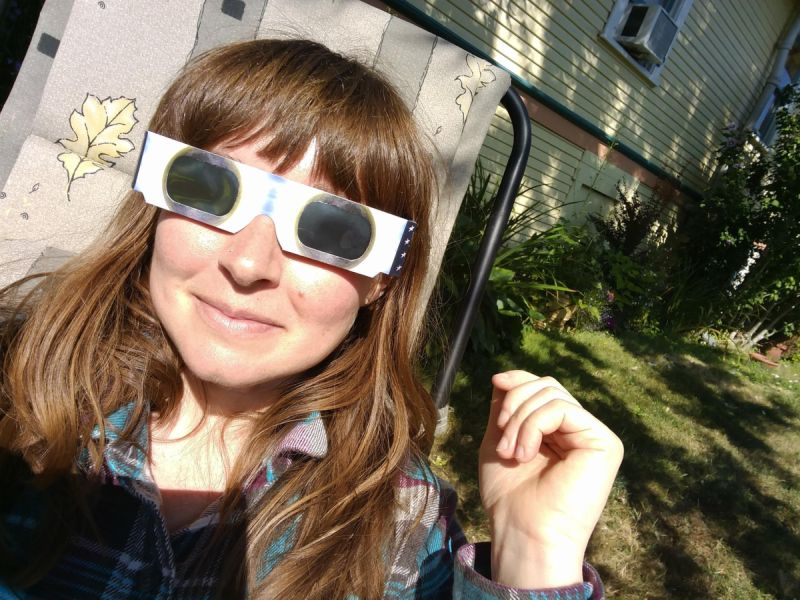
\includegraphics{img/Christy_eclipse.jpg}
\caption{title}
\end{figure}

    \begin{figure}
\centering
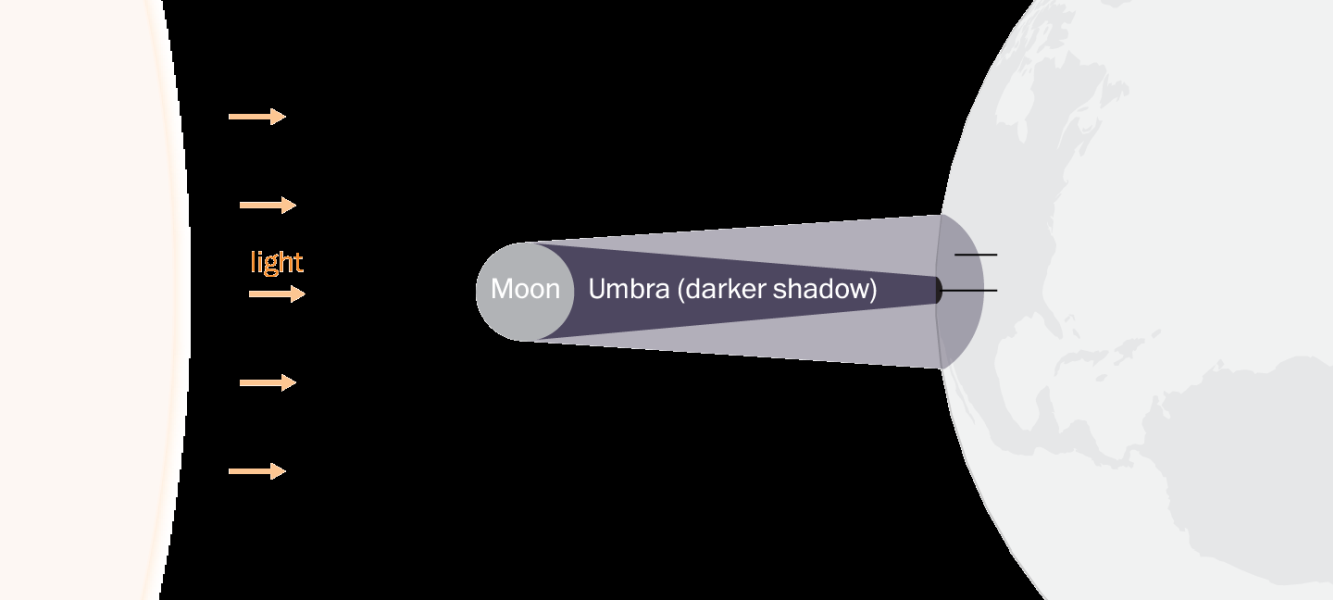
\includegraphics{img/_alignment-lines-720.png}
\caption{title}
\end{figure}

    \begin{figure}
\centering
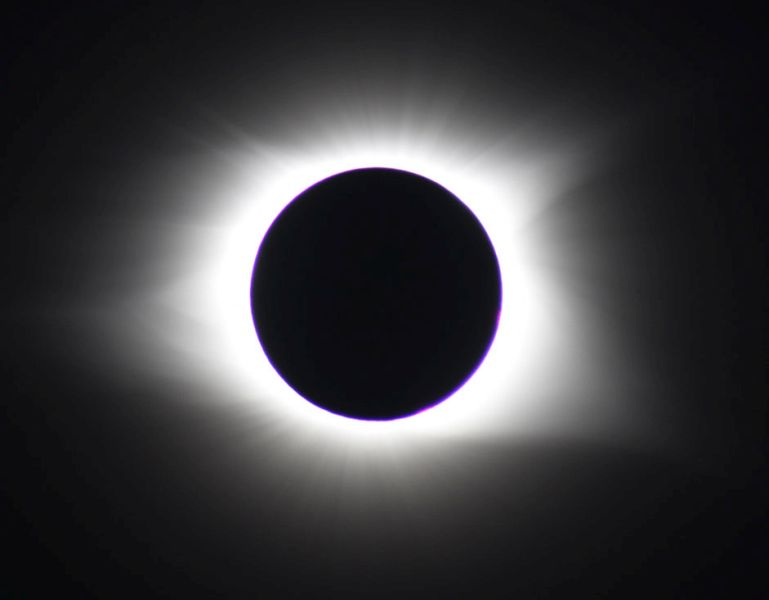
\includegraphics{img/Corona-2017-Aug-21-m.jpg}
\caption{title}
\end{figure}

    \hypertarget{we-can-use-python-and-jupyter-to-find-out}{%
\subsubsection{We can use Python and Jupyter to find
out:}\label{we-can-use-python-and-jupyter-to-find-out}}

\begin{enumerate}
\def\labelenumi{\arabic{enumi}.}
\item
  When and where will we be able to see an eclipse?
\item
  Which upcoming eclipse will pass over the most people?
\item
  What are the largest cities in that eclipse?
\end{enumerate}

    \hypertarget{python-mapping-libraries}{%
\section{Python Mapping Libraries}\label{python-mapping-libraries}}

    \hypertarget{matplotlib}{%
\subsection{\texorpdfstring{\href{https://matplotlib.org/}{Matplotlib}}{Matplotlib}}\label{matplotlib}}

\hypertarget{a-python-plotting-library-which-produces-publication-quality-maps-and-diagrams-in-both-static-and-interactive-formats.}{%
\paragraph{A Python plotting library which produces publication quality
maps and diagrams in both static and interactive
formats.}\label{a-python-plotting-library-which-produces-publication-quality-maps-and-diagrams-in-both-static-and-interactive-formats.}}

    \begin{Verbatim}[commandchars=\\\{\}]
{\color{incolor}In [{\color{incolor} }]:} \PY{o}{\PYZpc{}}\PY{k}{matplotlib} inline
        \PY{k+kn}{import} \PY{n+nn}{matplotlib}\PY{n+nn}{.}\PY{n+nn}{pyplot} \PY{k}{as} \PY{n+nn}{plt}
\end{Verbatim}


    \hypertarget{pandas}{%
\subsection{\texorpdfstring{\href{https://pandas.pydata.org/}{Pandas}}{Pandas}}\label{pandas}}

\hypertarget{provides-high-performance-easy-to-use-data-structures-and-data-analysis-tools}{%
\paragraph{Provides high-performance, easy-to-use data structures and
data analysis
tools}\label{provides-high-performance-easy-to-use-data-structures-and-data-analysis-tools}}

\hypertarget{geopandas}{%
\subsection{\texorpdfstring{\href{http://geopandas.org/}{GeoPandas}}{GeoPandas}}\label{geopandas}}

\hypertarget{geographically-enabled-pandas-depends-on-shapely-for-manipulation-and-analysis-of-planar-geometric-objects}{%
\paragraph{\texorpdfstring{Geographically-enabled Pandas, depends on
\href{https://github.com/Toblerity/Shapely}{Shapely} for manipulation
and analysis of planar geometric
objects}{Geographically-enabled Pandas, depends on Shapely for manipulation and analysis of planar geometric objects}}\label{geographically-enabled-pandas-depends-on-shapely-for-manipulation-and-analysis-of-planar-geometric-objects}}

    \begin{Verbatim}[commandchars=\\\{\}]
{\color{incolor}In [{\color{incolor} }]:} \PY{k+kn}{import} \PY{n+nn}{pandas} \PY{k}{as} \PY{n+nn}{pd}
        \PY{k+kn}{import} \PY{n+nn}{geopandas} \PY{k}{as} \PY{n+nn}{gpd}
\end{Verbatim}


    \hypertarget{lets-start-by-making-a-simple-map}{%
\section{Let's Start by Making a Simple
Map}\label{lets-start-by-making-a-simple-map}}

    \begin{Verbatim}[commandchars=\\\{\}]
{\color{incolor}In [{\color{incolor} }]:} \PY{c+c1}{\PYZsh{} GeoPandas comes with some data that we can quickly load in}
        \PY{n}{world} \PY{o}{=} \PY{n}{gpd}\PY{o}{.}\PY{n}{read\PYZus{}file}\PY{p}{(}\PY{n}{gpd}\PY{o}{.}\PY{n}{datasets}\PY{o}{.}\PY{n}{get\PYZus{}path}\PY{p}{(}\PY{l+s+s1}{\PYZsq{}}\PY{l+s+s1}{naturalearth\PYZus{}lowres}\PY{l+s+s1}{\PYZsq{}}\PY{p}{)}\PY{p}{)}
\end{Verbatim}


    \begin{Verbatim}[commandchars=\\\{\}]
{\color{incolor}In [{\color{incolor} }]:} \PY{c+c1}{\PYZsh{} And check out the top few rows \PYZhy{} notice it comes with attributes like population and GDP, }
        \PY{c+c1}{\PYZsh{} as well as geometry }
        \PY{n}{world}\PY{o}{.}\PY{n}{head}\PY{p}{(}\PY{p}{)}
\end{Verbatim}


    \begin{Verbatim}[commandchars=\\\{\}]
{\color{incolor}In [{\color{incolor} }]:} \PY{n}{world}\PY{o}{.}\PY{n}{crs}
\end{Verbatim}


    \begin{Verbatim}[commandchars=\\\{\}]
{\color{incolor}In [{\color{incolor} }]:} \PY{c+c1}{\PYZsh{} Use the plot method to view the spatial component}
        \PY{n}{world}\PY{o}{.}\PY{n}{plot}\PY{p}{(}\PY{p}{)}
\end{Verbatim}


    \begin{Verbatim}[commandchars=\\\{\}]
{\color{incolor}In [{\color{incolor} }]:} \PY{c+c1}{\PYZsh{} You\PYZsq{}ll usually want to customize how your map looks}
        \PY{n}{world}\PY{o}{.}\PY{n}{plot}\PY{p}{(}\PY{n}{color}\PY{o}{=}\PY{l+s+s1}{\PYZsq{}}\PY{l+s+s1}{grey}\PY{l+s+s1}{\PYZsq{}}\PY{p}{,} \PY{n}{linewidth}\PY{o}{=}\PY{l+m+mf}{0.5}\PY{p}{,} \PY{n}{edgecolor}\PY{o}{=}\PY{l+s+s1}{\PYZsq{}}\PY{l+s+s1}{white}\PY{l+s+s1}{\PYZsq{}}\PY{p}{,} \PY{n}{figsize}\PY{o}{=}\PY{p}{(}\PY{l+m+mi}{15}\PY{p}{,}\PY{l+m+mi}{10}\PY{p}{)}\PY{p}{)}
\end{Verbatim}


    \begin{Verbatim}[commandchars=\\\{\}]
{\color{incolor}In [{\color{incolor} }]:} \PY{c+c1}{\PYZsh{} We\PYZsq{}ll need to load in some local data}
        \PY{k+kn}{import} \PY{n+nn}{os}
        \PY{n}{data\PYZus{}pth} \PY{o}{=} \PY{l+s+s2}{\PYZdq{}}\PY{l+s+s2}{../Data/}\PY{l+s+s2}{\PYZdq{}} 
\end{Verbatim}


    \begin{Verbatim}[commandchars=\\\{\}]
{\color{incolor}In [{\color{incolor} }]:} \PY{c+c1}{\PYZsh{} GeoPandas comes with city data, but its just the capital cities, so I\PYZsq{}ll load in my own}
        \PY{n}{cities} \PY{o}{=} \PY{n}{gpd}\PY{o}{.}\PY{n}{read\PYZus{}file}\PY{p}{(}\PY{n}{os}\PY{o}{.}\PY{n}{path}\PY{o}{.}\PY{n}{join}\PY{p}{(}\PY{n}{data\PYZus{}pth}\PY{p}{,} \PY{l+s+s2}{\PYZdq{}}\PY{l+s+s2}{ne\PYZus{}10m\PYZus{}populated\PYZus{}places.shp}\PY{l+s+s2}{\PYZdq{}}\PY{p}{)}\PY{p}{)}
\end{Verbatim}


    \begin{Verbatim}[commandchars=\\\{\}]
{\color{incolor}In [{\color{incolor} }]:} \PY{c+c1}{\PYZsh{} View the top few rows}
        \PY{n}{cities}\PY{o}{.}\PY{n}{head}\PY{p}{(}\PY{p}{)}
\end{Verbatim}


    \begin{Verbatim}[commandchars=\\\{\}]
{\color{incolor}In [{\color{incolor} }]:} \PY{n}{cities}\PY{o}{.}\PY{n}{crs}
\end{Verbatim}


    \begin{Verbatim}[commandchars=\\\{\}]
{\color{incolor}In [{\color{incolor} }]:} \PY{c+c1}{\PYZsh{} And plot to view the spatial component}
        \PY{n}{cities}\PY{o}{.}\PY{n}{plot}\PY{p}{(}\PY{n}{figsize}\PY{o}{=}\PY{p}{(}\PY{l+m+mi}{15}\PY{p}{,}\PY{l+m+mi}{10}\PY{p}{)}\PY{p}{,} \PY{n}{color}\PY{o}{=}\PY{l+s+s1}{\PYZsq{}}\PY{l+s+s1}{orange}\PY{l+s+s1}{\PYZsq{}}\PY{p}{,} \PY{n}{markersize}\PY{o}{=}\PY{l+m+mi}{5}\PY{p}{)}
\end{Verbatim}


    \begin{Verbatim}[commandchars=\\\{\}]
{\color{incolor}In [{\color{incolor} }]:} \PY{n}{world}\PY{o}{.}\PY{n}{crs} \PY{o}{==} \PY{n}{cities}\PY{o}{.}\PY{n}{crs}
\end{Verbatim}


    \begin{Verbatim}[commandchars=\\\{\}]
{\color{incolor}In [{\color{incolor} }]:} \PY{n}{base} \PY{o}{=} \PY{n}{world}\PY{o}{.}\PY{n}{plot}\PY{p}{(}\PY{n}{color}\PY{o}{=}\PY{l+s+s1}{\PYZsq{}}\PY{l+s+s1}{grey}\PY{l+s+s1}{\PYZsq{}}\PY{p}{,} \PY{n}{linewidth}\PY{o}{=}\PY{l+m+mf}{0.5}\PY{p}{,} \PY{n}{edgecolor}\PY{o}{=}\PY{l+s+s1}{\PYZsq{}}\PY{l+s+s1}{white}\PY{l+s+s1}{\PYZsq{}}\PY{p}{,} \PY{n}{figsize}\PY{o}{=}\PY{p}{(}\PY{l+m+mi}{15}\PY{p}{,}\PY{l+m+mi}{10}\PY{p}{)}\PY{p}{)}
        \PY{n}{cities}\PY{o}{.}\PY{n}{plot}\PY{p}{(}\PY{n}{ax}\PY{o}{=}\PY{n}{base}\PY{p}{,} \PY{n}{color}\PY{o}{=}\PY{l+s+s1}{\PYZsq{}}\PY{l+s+s1}{orange}\PY{l+s+s1}{\PYZsq{}}\PY{p}{,} \PY{n}{markersize}\PY{o}{=}\PY{l+m+mi}{5}\PY{p}{)}
        \PY{n}{base}\PY{o}{.}\PY{n}{set\PYZus{}axis\PYZus{}off}\PY{p}{(}\PY{p}{)} 
\end{Verbatim}


    \hypertarget{what-do-we-want-to-know}{%
\subsubsection{What do we want to know?}\label{what-do-we-want-to-know}}

\begin{enumerate}
\def\labelenumi{\arabic{enumi}.}
\tightlist
\item
  When and where will we be able to see an eclipse?
\end{enumerate}

    \begin{Verbatim}[commandchars=\\\{\}]
{\color{incolor}In [{\color{incolor} }]:} \PY{c+c1}{\PYZsh{} Load in Eclipse data}
        \PY{n}{eclipses} \PY{o}{=} \PY{n}{gpd}\PY{o}{.}\PY{n}{read\PYZus{}file}\PY{p}{(}\PY{n}{os}\PY{o}{.}\PY{n}{path}\PY{o}{.}\PY{n}{join}\PY{p}{(}\PY{n}{data\PYZus{}pth}\PY{p}{,} \PY{l+s+s2}{\PYZdq{}}\PY{l+s+s2}{Eclipses.shp}\PY{l+s+s2}{\PYZdq{}}\PY{p}{)}\PY{p}{)}
\end{Verbatim}


    \begin{Verbatim}[commandchars=\\\{\}]
{\color{incolor}In [{\color{incolor} }]:} \PY{c+c1}{\PYZsh{} Examine the first few rows}
        \PY{n}{eclipses}\PY{o}{.}\PY{n}{head}\PY{p}{(}\PY{p}{)}
\end{Verbatim}


    \begin{Verbatim}[commandchars=\\\{\}]
{\color{incolor}In [{\color{incolor} }]:} \PY{c+c1}{\PYZsh{} Check the coorindate reference system}
        \PY{n}{eclipses}\PY{o}{.}\PY{n}{crs}
\end{Verbatim}


    \begin{Verbatim}[commandchars=\\\{\}]
{\color{incolor}In [{\color{incolor} }]:} \PY{c+c1}{\PYZsh{} And let\PYZsq{}s plot with a customized style}
        \PY{n}{eclipses}\PY{o}{.}\PY{n}{plot}\PY{p}{(}\PY{n}{figsize}\PY{o}{=}\PY{p}{(}\PY{l+m+mi}{15}\PY{p}{,}\PY{l+m+mi}{10}\PY{p}{)}\PY{p}{,} \PY{n}{color}\PY{o}{=}\PY{l+s+s1}{\PYZsq{}}\PY{l+s+s1}{black}\PY{l+s+s1}{\PYZsq{}}\PY{p}{,} \PY{n}{edgecolor}\PY{o}{=}\PY{l+s+s1}{\PYZsq{}}\PY{l+s+s1}{yellow}\PY{l+s+s1}{\PYZsq{}}\PY{p}{,} \PY{n}{alpha}\PY{o}{=}\PY{l+m+mf}{0.75}\PY{p}{)}
\end{Verbatim}


    \begin{Verbatim}[commandchars=\\\{\}]
{\color{incolor}In [{\color{incolor} }]:} \PY{c+c1}{\PYZsh{} GeoPandas let\PYZsq{}s you plot the minimum bounding box of each entity}
        \PY{n}{eclipses}\PY{o}{.}\PY{n}{envelope}\PY{o}{.}\PY{n}{plot}\PY{p}{(}\PY{n}{figsize}\PY{o}{=}\PY{p}{(}\PY{l+m+mi}{15}\PY{p}{,}\PY{l+m+mi}{10}\PY{p}{)}\PY{p}{)}
\end{Verbatim}


    \begin{Verbatim}[commandchars=\\\{\}]
{\color{incolor}In [{\color{incolor} }]:} \PY{c+c1}{\PYZsh{} Let\PYZsq{}s plot the eclipses on top of our world data}
        \PY{n}{base} \PY{o}{=} \PY{n}{world}\PY{o}{.}\PY{n}{plot}\PY{p}{(}\PY{n}{color}\PY{o}{=}\PY{l+s+s1}{\PYZsq{}}\PY{l+s+s1}{lightgrey}\PY{l+s+s1}{\PYZsq{}}\PY{p}{,} \PY{n}{linewidth}\PY{o}{=}\PY{l+m+mf}{0.5}\PY{p}{,} \PY{n}{edgecolor}\PY{o}{=}\PY{l+s+s1}{\PYZsq{}}\PY{l+s+s1}{white}\PY{l+s+s1}{\PYZsq{}}\PY{p}{,} \PY{n}{figsize}\PY{o}{=}\PY{p}{(}\PY{l+m+mi}{15}\PY{p}{,}\PY{l+m+mi}{10}\PY{p}{)}\PY{p}{)}
        \PY{n}{eclipses}\PY{o}{.}\PY{n}{plot}\PY{p}{(}\PY{n}{ax}\PY{o}{=}\PY{n}{base}\PY{p}{,} \PY{n}{color}\PY{o}{=}\PY{l+s+s1}{\PYZsq{}}\PY{l+s+s1}{black}\PY{l+s+s1}{\PYZsq{}}\PY{p}{,} \PY{n}{edgecolor}\PY{o}{=}\PY{l+s+s1}{\PYZsq{}}\PY{l+s+s1}{yellow}\PY{l+s+s1}{\PYZsq{}}\PY{p}{,} \PY{n}{alpha}\PY{o}{=}\PY{l+m+mf}{0.75}\PY{p}{)}
        \PY{n}{base}\PY{o}{.}\PY{n}{set\PYZus{}axis\PYZus{}off}\PY{p}{(}\PY{p}{)}
\end{Verbatim}


    \begin{Verbatim}[commandchars=\\\{\}]
{\color{incolor}In [{\color{incolor} }]:} \PY{c+c1}{\PYZsh{} But how do we know which is which?}
        \PY{n}{base} \PY{o}{=} \PY{n}{world}\PY{o}{.}\PY{n}{plot}\PY{p}{(}\PY{n}{color}\PY{o}{=}\PY{l+s+s1}{\PYZsq{}}\PY{l+s+s1}{lightgrey}\PY{l+s+s1}{\PYZsq{}}\PY{p}{,} \PY{n}{linewidth}\PY{o}{=}\PY{l+m+mf}{0.5}\PY{p}{,} \PY{n}{edgecolor}\PY{o}{=}\PY{l+s+s1}{\PYZsq{}}\PY{l+s+s1}{white}\PY{l+s+s1}{\PYZsq{}}\PY{p}{,} \PY{n}{figsize}\PY{o}{=}\PY{p}{(}\PY{l+m+mi}{15}\PY{p}{,}\PY{l+m+mi}{10}\PY{p}{)}\PY{p}{)}
        
        \PY{c+c1}{\PYZsh{} We can add a catetorical value and set the column to Year. We can also add a legend.}
        \PY{n}{eclipses}\PY{o}{.}\PY{n}{plot}\PY{p}{(}\PY{n}{ax}\PY{o}{=}\PY{n}{base}\PY{p}{,} \PY{n}{cmap}\PY{o}{=}\PY{l+s+s1}{\PYZsq{}}\PY{l+s+s1}{tab10}\PY{l+s+s1}{\PYZsq{}}\PY{p}{,} \PY{n}{alpha}\PY{o}{=}\PY{l+m+mf}{0.5}\PY{p}{,} \PY{n}{categorical} \PY{o}{=} \PY{k+kc}{True}\PY{p}{,} \PY{n}{column} \PY{o}{=} \PY{l+s+s2}{\PYZdq{}}\PY{l+s+s2}{Year}\PY{l+s+s2}{\PYZdq{}}\PY{p}{,} \PY{n}{legend}\PY{o}{=}\PY{k+kc}{True}\PY{p}{)}
        \PY{n}{base}\PY{o}{.}\PY{n}{set\PYZus{}axis\PYZus{}off}\PY{p}{(}\PY{p}{)}
        \PY{n}{base}\PY{o}{.}\PY{n}{get\PYZus{}legend}\PY{p}{(}\PY{p}{)}\PY{o}{.}\PY{n}{set\PYZus{}bbox\PYZus{}to\PYZus{}anchor}\PY{p}{(}\PY{p}{(}\PY{o}{.}\PY{l+m+mi}{05}\PY{p}{,}\PY{o}{.}\PY{l+m+mi}{7}\PY{p}{)}\PY{p}{)}
\end{Verbatim}


    \hypertarget{what-do-we-want-to-know}{%
\subsubsection{What do we want to know?}\label{what-do-we-want-to-know}}

\begin{enumerate}
\def\labelenumi{\arabic{enumi}.}
\item
  When and where will we be able to see an eclipse?
\item
  What upcoming eclipse will pass over the most people?
\end{enumerate}

    \begin{Verbatim}[commandchars=\\\{\}]
{\color{incolor}In [{\color{incolor} }]:} \PY{c+c1}{\PYZsh{} Is the cities data still in the same crs as the eclipse data? It needs to be to plot correctly!}
        \PY{n}{world}\PY{o}{.}\PY{n}{crs} \PY{o}{==} \PY{n}{eclipses}\PY{o}{.}\PY{n}{crs} \PY{o}{==} \PY{n}{cities}\PY{o}{.}\PY{n}{crs}
\end{Verbatim}


    \begin{Verbatim}[commandchars=\\\{\}]
{\color{incolor}In [{\color{incolor} }]:} \PY{c+c1}{\PYZsh{} Now we\PYZsq{}ll plot our basemap, our eclipse paths, and our cities}
        \PY{n}{base} \PY{o}{=} \PY{n}{world}\PY{o}{.}\PY{n}{plot}\PY{p}{(}\PY{n}{color}\PY{o}{=}\PY{l+s+s1}{\PYZsq{}}\PY{l+s+s1}{lightgrey}\PY{l+s+s1}{\PYZsq{}}\PY{p}{,} \PY{n}{linewidth}\PY{o}{=}\PY{l+m+mf}{0.5}\PY{p}{,} \PY{n}{edgecolor}\PY{o}{=}\PY{l+s+s1}{\PYZsq{}}\PY{l+s+s1}{white}\PY{l+s+s1}{\PYZsq{}}\PY{p}{,} \PY{n}{figsize}\PY{o}{=}\PY{p}{(}\PY{l+m+mi}{15}\PY{p}{,}\PY{l+m+mi}{10}\PY{p}{)}\PY{p}{)}
        \PY{n}{eclipses}\PY{o}{.}\PY{n}{plot}\PY{p}{(}\PY{n}{ax}\PY{o}{=}\PY{n}{base}\PY{p}{,} \PY{n}{color}\PY{o}{=}\PY{l+s+s1}{\PYZsq{}}\PY{l+s+s1}{black}\PY{l+s+s1}{\PYZsq{}}\PY{p}{,} \PY{n}{edgecolor}\PY{o}{=}\PY{l+s+s1}{\PYZsq{}}\PY{l+s+s1}{yellow}\PY{l+s+s1}{\PYZsq{}}\PY{p}{,} \PY{n}{alpha}\PY{o}{=}\PY{l+m+mf}{0.75}\PY{p}{)}
        \PY{n}{cities}\PY{o}{.}\PY{n}{plot}\PY{p}{(}\PY{n}{ax}\PY{o}{=}\PY{n}{base}\PY{p}{,} \PY{n}{color}\PY{o}{=}\PY{l+s+s1}{\PYZsq{}}\PY{l+s+s1}{orange}\PY{l+s+s1}{\PYZsq{}}\PY{p}{,} \PY{n}{markersize}\PY{o}{=}\PY{l+m+mi}{5}\PY{p}{)}
        \PY{n}{base}\PY{o}{.}\PY{n}{set\PYZus{}axis\PYZus{}off}\PY{p}{(}\PY{p}{)}
\end{Verbatim}


    \begin{Verbatim}[commandchars=\\\{\}]
{\color{incolor}In [{\color{incolor} }]:} \PY{c+c1}{\PYZsh{} Start by getting all the cities that intersect any eclipse, a spatial join using the geom column}
        \PY{n}{allecities} \PY{o}{=} \PY{n}{gpd}\PY{o}{.}\PY{n}{sjoin}\PY{p}{(}\PY{n}{cities}\PY{p}{,} \PY{n}{eclipses}\PY{p}{,} \PY{n}{how}\PY{o}{=}\PY{l+s+s1}{\PYZsq{}}\PY{l+s+s1}{inner}\PY{l+s+s1}{\PYZsq{}}\PY{p}{,} \PY{n}{op}\PY{o}{=}\PY{l+s+s1}{\PYZsq{}}\PY{l+s+s1}{intersects}\PY{l+s+s1}{\PYZsq{}}\PY{p}{)}
\end{Verbatim}


    \begin{Verbatim}[commandchars=\\\{\}]
{\color{incolor}In [{\color{incolor} }]:} \PY{n}{allecities}\PY{o}{.}\PY{n}{head}\PY{p}{(}\PY{p}{)}
\end{Verbatim}


    \begin{Verbatim}[commandchars=\\\{\}]
{\color{incolor}In [{\color{incolor} }]:} \PY{n}{allecities} \PY{o}{=} \PY{n}{pd}\PY{o}{.}\PY{n}{DataFrame}\PY{p}{(}\PY{n}{allecities}\PY{p}{[}\PY{p}{[}\PY{l+s+s1}{\PYZsq{}}\PY{l+s+s1}{POP}\PY{l+s+s1}{\PYZsq{}}\PY{p}{,} \PY{l+s+s1}{\PYZsq{}}\PY{l+s+s1}{Year}\PY{l+s+s1}{\PYZsq{}}\PY{p}{]}\PY{p}{]}\PY{p}{)}
\end{Verbatim}


    \begin{Verbatim}[commandchars=\\\{\}]
{\color{incolor}In [{\color{incolor} }]:} \PY{n}{allecities}\PY{o}{.}\PY{n}{head}\PY{p}{(}\PY{p}{)}
\end{Verbatim}


    \begin{Verbatim}[commandchars=\\\{\}]
{\color{incolor}In [{\color{incolor} }]:} \PY{c+c1}{\PYZsh{} Create a temporary variable to hold our years and populations}
        \PY{n}{temp\PYZus{}group} \PY{o}{=} \PY{n}{allecities}\PY{o}{.}\PY{n}{groupby}\PY{p}{(}\PY{p}{[}\PY{l+s+s1}{\PYZsq{}}\PY{l+s+s1}{Year}\PY{l+s+s1}{\PYZsq{}}\PY{p}{]}\PY{p}{)}\PY{p}{[}\PY{p}{[}\PY{l+s+s2}{\PYZdq{}}\PY{l+s+s2}{POP}\PY{l+s+s2}{\PYZdq{}}\PY{p}{]}\PY{p}{]}\PY{o}{.}\PY{n}{sum}\PY{p}{(}\PY{p}{)}
\end{Verbatim}


    \begin{Verbatim}[commandchars=\\\{\}]
{\color{incolor}In [{\color{incolor} }]:} \PY{n}{temp\PYZus{}group}
\end{Verbatim}


    \begin{Verbatim}[commandchars=\\\{\}]
{\color{incolor}In [{\color{incolor} }]:} \PY{c+c1}{\PYZsh{} Add that column to our eclipse data, joining on the Year column}
        \PY{n}{eclipses\PYZus{}pop} \PY{o}{=} \PY{n}{pd}\PY{o}{.}\PY{n}{merge}\PY{p}{(}\PY{n}{eclipses}\PY{p}{,} \PY{n}{temp\PYZus{}group}\PY{p}{,} \PY{n}{left\PYZus{}on}\PY{o}{=}\PY{l+s+s1}{\PYZsq{}}\PY{l+s+s1}{Year}\PY{l+s+s1}{\PYZsq{}}\PY{p}{,} \PY{n}{right\PYZus{}index}\PY{o}{=}\PY{k+kc}{True}\PY{p}{)}
\end{Verbatim}


    \begin{Verbatim}[commandchars=\\\{\}]
{\color{incolor}In [{\color{incolor} }]:} \PY{c+c1}{\PYZsh{} Now we have populations associated with each eclipse}
        \PY{n}{eclipses\PYZus{}pop}\PY{o}{.}\PY{n}{head}\PY{p}{(}\PY{p}{)}
\end{Verbatim}


    \begin{Verbatim}[commandchars=\\\{\}]
{\color{incolor}In [{\color{incolor} }]:} \PY{c+c1}{\PYZsh{} Sort the results to find out which eclipse will cover the most people}
        \PY{n}{eclipses\PYZus{}pop}\PY{o}{.}\PY{n}{sort\PYZus{}values}\PY{p}{(}\PY{l+s+s1}{\PYZsq{}}\PY{l+s+s1}{POP}\PY{l+s+s1}{\PYZsq{}}\PY{p}{,} \PY{n}{ascending} \PY{o}{=} \PY{k+kc}{False}\PY{p}{)}
\end{Verbatim}


    \begin{Verbatim}[commandchars=\\\{\}]
{\color{incolor}In [{\color{incolor} }]:} \PY{c+c1}{\PYZsh{} Let\PYZsq{}s plot this}
        \PY{n}{base} \PY{o}{=} \PY{n}{world}\PY{o}{.}\PY{n}{plot}\PY{p}{(}\PY{n}{color}\PY{o}{=}\PY{l+s+s1}{\PYZsq{}}\PY{l+s+s1}{lightgrey}\PY{l+s+s1}{\PYZsq{}}\PY{p}{,} \PY{n}{linewidth}\PY{o}{=}\PY{l+m+mf}{0.5}\PY{p}{,} \PY{n}{edgecolor}\PY{o}{=}\PY{l+s+s1}{\PYZsq{}}\PY{l+s+s1}{white}\PY{l+s+s1}{\PYZsq{}}\PY{p}{,} \PY{n}{figsize}\PY{o}{=}\PY{p}{(}\PY{l+m+mi}{15}\PY{p}{,}\PY{l+m+mi}{10}\PY{p}{)}\PY{p}{)}
        \PY{n}{eclipses\PYZus{}pop}\PY{o}{.}\PY{n}{plot}\PY{p}{(}\PY{n}{ax}\PY{o}{=}\PY{n}{base}\PY{p}{,} \PY{n}{cmap}\PY{o}{=}\PY{l+s+s1}{\PYZsq{}}\PY{l+s+s1}{Oranges}\PY{l+s+s1}{\PYZsq{}}\PY{p}{,} \PY{n}{alpha}\PY{o}{=}\PY{l+m+mf}{0.5}\PY{p}{,} \PY{n}{column} \PY{o}{=} \PY{l+s+s2}{\PYZdq{}}\PY{l+s+s2}{POP}\PY{l+s+s2}{\PYZdq{}}\PY{p}{)}
        \PY{n}{base}\PY{o}{.}\PY{n}{set\PYZus{}axis\PYZus{}off}\PY{p}{(}\PY{p}{)}
\end{Verbatim}


    \begin{Verbatim}[commandchars=\\\{\}]
{\color{incolor}In [{\color{incolor} }]:} \PY{c+c1}{\PYZsh{} As we saw earlier, this eclipse is happening in 2024}
        \PY{n}{base} \PY{o}{=} \PY{n}{world}\PY{o}{.}\PY{n}{plot}\PY{p}{(}\PY{n}{color}\PY{o}{=}\PY{l+s+s1}{\PYZsq{}}\PY{l+s+s1}{lightgrey}\PY{l+s+s1}{\PYZsq{}}\PY{p}{,} \PY{n}{linewidth}\PY{o}{=}\PY{l+m+mf}{0.5}\PY{p}{,} \PY{n}{edgecolor}\PY{o}{=}\PY{l+s+s1}{\PYZsq{}}\PY{l+s+s1}{white}\PY{l+s+s1}{\PYZsq{}}\PY{p}{,} \PY{n}{figsize}\PY{o}{=}\PY{p}{(}\PY{l+m+mi}{15}\PY{p}{,}\PY{l+m+mi}{10}\PY{p}{)}\PY{p}{)}
        \PY{n}{eclipses}\PY{o}{.}\PY{n}{plot}\PY{p}{(}\PY{n}{ax}\PY{o}{=}\PY{n}{base}\PY{p}{,} \PY{n}{cmap}\PY{o}{=}\PY{l+s+s1}{\PYZsq{}}\PY{l+s+s1}{tab10}\PY{l+s+s1}{\PYZsq{}}\PY{p}{,} \PY{n}{alpha}\PY{o}{=}\PY{l+m+mf}{0.5}\PY{p}{,} \PY{n}{categorical} \PY{o}{=} \PY{k+kc}{True}\PY{p}{,} \PY{n}{column} \PY{o}{=} \PY{l+s+s2}{\PYZdq{}}\PY{l+s+s2}{Year}\PY{l+s+s2}{\PYZdq{}}\PY{p}{,} \PY{n}{legend}\PY{o}{=}\PY{k+kc}{True}\PY{p}{)}
        \PY{n}{base}\PY{o}{.}\PY{n}{set\PYZus{}axis\PYZus{}off}\PY{p}{(}\PY{p}{)}
        \PY{n}{base}\PY{o}{.}\PY{n}{get\PYZus{}legend}\PY{p}{(}\PY{p}{)}\PY{o}{.}\PY{n}{set\PYZus{}bbox\PYZus{}to\PYZus{}anchor}\PY{p}{(}\PY{p}{(}\PY{o}{.}\PY{l+m+mi}{05}\PY{p}{,}\PY{o}{.}\PY{l+m+mi}{7}\PY{p}{)}\PY{p}{)}
\end{Verbatim}


    \hypertarget{what-do-we-want-to-know}{%
\subsubsection{What do we want to know?}\label{what-do-we-want-to-know}}

\begin{enumerate}
\def\labelenumi{\arabic{enumi}.}
\item
  When and where will we be able to see an eclipse?
\item
  What upcoming eclipse will pass over the most people?
\item
  What are the largest cities in that eclipse?
\end{enumerate}

    \begin{Verbatim}[commandchars=\\\{\}]
{\color{incolor}In [{\color{incolor} }]:} \PY{c+c1}{\PYZsh{} Let\PYZsq{}s assign the 2024 eclipse to its own variable}
        \PY{n}{myeclipse} \PY{o}{=} \PY{n}{eclipses}\PY{p}{[}\PY{p}{(}\PY{n}{eclipses}\PY{p}{[}\PY{l+s+s1}{\PYZsq{}}\PY{l+s+s1}{Year}\PY{l+s+s1}{\PYZsq{}}\PY{p}{]} \PY{o}{==} \PY{l+m+mi}{2024}\PY{p}{)}\PY{p}{]}
\end{Verbatim}


    \begin{Verbatim}[commandchars=\\\{\}]
{\color{incolor}In [{\color{incolor} }]:} \PY{c+c1}{\PYZsh{} Let\PYZsq{}s plot it }
        \PY{n}{base} \PY{o}{=} \PY{n}{world}\PY{o}{.}\PY{n}{plot}\PY{p}{(}\PY{n}{color}\PY{o}{=}\PY{l+s+s1}{\PYZsq{}}\PY{l+s+s1}{lightgrey}\PY{l+s+s1}{\PYZsq{}}\PY{p}{,} \PY{n}{linewidth}\PY{o}{=}\PY{l+m+mf}{0.5}\PY{p}{,} \PY{n}{edgecolor}\PY{o}{=}\PY{l+s+s1}{\PYZsq{}}\PY{l+s+s1}{white}\PY{l+s+s1}{\PYZsq{}}\PY{p}{,} \PY{n}{figsize}\PY{o}{=}\PY{p}{(}\PY{l+m+mi}{15}\PY{p}{,}\PY{l+m+mi}{10}\PY{p}{)}\PY{p}{)}
        \PY{n}{myeclipse}\PY{o}{.}\PY{n}{plot}\PY{p}{(}\PY{n}{ax}\PY{o}{=}\PY{n}{base}\PY{p}{,} \PY{n}{color}\PY{o}{=}\PY{l+s+s1}{\PYZsq{}}\PY{l+s+s1}{black}\PY{l+s+s1}{\PYZsq{}}\PY{p}{,} \PY{n}{edgecolor}\PY{o}{=}\PY{l+s+s1}{\PYZsq{}}\PY{l+s+s1}{yellow}\PY{l+s+s1}{\PYZsq{}}\PY{p}{,} \PY{n}{alpha}\PY{o}{=}\PY{l+m+mf}{0.75}\PY{p}{)}
        \PY{n}{cities}\PY{o}{.}\PY{n}{plot}\PY{p}{(}\PY{n}{marker}\PY{o}{=}\PY{l+s+s1}{\PYZsq{}}\PY{l+s+s1}{*}\PY{l+s+s1}{\PYZsq{}}\PY{p}{,} \PY{n}{color}\PY{o}{=}\PY{l+s+s1}{\PYZsq{}}\PY{l+s+s1}{orange}\PY{l+s+s1}{\PYZsq{}}\PY{p}{,} \PY{n}{markersize}\PY{o}{=}\PY{l+m+mi}{5}\PY{p}{,} \PY{n}{ax}\PY{o}{=}\PY{n}{base}\PY{p}{)}
        \PY{n}{base}\PY{o}{.}\PY{n}{set\PYZus{}axis\PYZus{}off}\PY{p}{(}\PY{p}{)}
\end{Verbatim}


    \begin{Verbatim}[commandchars=\\\{\}]
{\color{incolor}In [{\color{incolor} }]:} \PY{c+c1}{\PYZsh{} Plot again, but this time I want to zoom in on that eclipse path}
        \PY{n}{base} \PY{o}{=} \PY{n}{world}\PY{o}{.}\PY{n}{plot}\PY{p}{(}\PY{n}{color}\PY{o}{=}\PY{l+s+s1}{\PYZsq{}}\PY{l+s+s1}{lightgrey}\PY{l+s+s1}{\PYZsq{}}\PY{p}{,} \PY{n}{linewidth}\PY{o}{=}\PY{l+m+mf}{0.5}\PY{p}{,} \PY{n}{edgecolor}\PY{o}{=}\PY{l+s+s1}{\PYZsq{}}\PY{l+s+s1}{white}\PY{l+s+s1}{\PYZsq{}}\PY{p}{,} \PY{n}{figsize}\PY{o}{=}\PY{p}{(}\PY{l+m+mi}{15}\PY{p}{,}\PY{l+m+mi}{10}\PY{p}{)}\PY{p}{)}
        \PY{n}{myeclipse}\PY{o}{.}\PY{n}{plot}\PY{p}{(}\PY{n}{ax}\PY{o}{=}\PY{n}{base}\PY{p}{,} \PY{n}{color}\PY{o}{=}\PY{l+s+s1}{\PYZsq{}}\PY{l+s+s1}{black}\PY{l+s+s1}{\PYZsq{}}\PY{p}{,} \PY{n}{edgecolor}\PY{o}{=}\PY{l+s+s1}{\PYZsq{}}\PY{l+s+s1}{yellow}\PY{l+s+s1}{\PYZsq{}}\PY{p}{,} \PY{n}{alpha}\PY{o}{=}\PY{l+m+mf}{0.75}\PY{p}{)}
        \PY{n}{cities}\PY{o}{.}\PY{n}{plot}\PY{p}{(}\PY{n}{marker}\PY{o}{=}\PY{l+s+s1}{\PYZsq{}}\PY{l+s+s1}{*}\PY{l+s+s1}{\PYZsq{}}\PY{p}{,} \PY{n}{color}\PY{o}{=}\PY{l+s+s1}{\PYZsq{}}\PY{l+s+s1}{orange}\PY{l+s+s1}{\PYZsq{}}\PY{p}{,} \PY{n}{markersize}\PY{o}{=}\PY{l+m+mi}{5}\PY{p}{,} \PY{n}{ax}\PY{o}{=}\PY{n}{base}\PY{p}{)}
        \PY{n}{bounds} \PY{o}{=} \PY{n}{myeclipse}\PY{o}{.}\PY{n}{geometry}\PY{o}{.}\PY{n}{bounds}
        \PY{n}{plt}\PY{o}{.}\PY{n}{xlim}\PY{p}{(}\PY{p}{[}\PY{n}{bounds}\PY{o}{.}\PY{n}{minx}\PY{o}{.}\PY{n}{min}\PY{p}{(}\PY{p}{)}\PY{o}{\PYZhy{}}\PY{l+m+mi}{5}\PY{p}{,} \PY{n}{bounds}\PY{o}{.}\PY{n}{maxx}\PY{o}{.}\PY{n}{max}\PY{p}{(}\PY{p}{)}\PY{o}{+}\PY{l+m+mi}{5}\PY{p}{]}\PY{p}{)}
        \PY{n}{plt}\PY{o}{.}\PY{n}{ylim}\PY{p}{(}\PY{p}{[}\PY{n}{bounds}\PY{o}{.}\PY{n}{miny}\PY{o}{.}\PY{n}{min}\PY{p}{(}\PY{p}{)}\PY{o}{\PYZhy{}}\PY{l+m+mi}{5}\PY{p}{,} \PY{n}{bounds}\PY{o}{.}\PY{n}{maxy}\PY{o}{.}\PY{n}{max}\PY{p}{(}\PY{p}{)}\PY{o}{+}\PY{l+m+mi}{5}\PY{p}{]}\PY{p}{)}
        \PY{n}{base}\PY{o}{.}\PY{n}{set\PYZus{}axis\PYZus{}off}\PY{p}{(}\PY{p}{)}
\end{Verbatim}


    \begin{Verbatim}[commandchars=\\\{\}]
{\color{incolor}In [{\color{incolor} }]:} \PY{c+c1}{\PYZsh{} Let\PYZsq{}s style the plot so that the eclipse looks eclipse\PYZhy{}ier}
        \PY{n}{base} \PY{o}{=} \PY{n}{world}\PY{o}{.}\PY{n}{plot}\PY{p}{(}\PY{n}{color}\PY{o}{=}\PY{l+s+s1}{\PYZsq{}}\PY{l+s+s1}{lightgray}\PY{l+s+s1}{\PYZsq{}}\PY{p}{,} \PY{n}{linewidth}\PY{o}{=}\PY{l+m+mf}{0.5}\PY{p}{,} \PY{n}{edgecolor}\PY{o}{=}\PY{l+s+s1}{\PYZsq{}}\PY{l+s+s1}{white}\PY{l+s+s1}{\PYZsq{}}\PY{p}{,} \PY{n}{figsize}\PY{o}{=}\PY{p}{(}\PY{l+m+mi}{15}\PY{p}{,}\PY{l+m+mi}{10}\PY{p}{)}\PY{p}{)}
        \PY{n}{myeclipse}\PY{o}{.}\PY{n}{plot}\PY{p}{(}\PY{n}{ax}\PY{o}{=}\PY{n}{base}\PY{p}{,} \PY{n}{color}\PY{o}{=}\PY{l+s+s1}{\PYZsq{}}\PY{l+s+s1}{black}\PY{l+s+s1}{\PYZsq{}}\PY{p}{,} \PY{n}{edgecolor}\PY{o}{=}\PY{l+s+s1}{\PYZsq{}}\PY{l+s+s1}{yellow}\PY{l+s+s1}{\PYZsq{}}\PY{p}{,} \PY{n}{alpha}\PY{o}{=}\PY{l+m+mf}{0.75}\PY{p}{)}
        \PY{n}{cities}\PY{o}{.}\PY{n}{plot}\PY{p}{(}\PY{n}{ax}\PY{o}{=}\PY{n}{base}\PY{p}{,} \PY{n}{color}\PY{o}{=}\PY{l+s+s1}{\PYZsq{}}\PY{l+s+s1}{black}\PY{l+s+s1}{\PYZsq{}}\PY{p}{,} \PY{n}{markersize}\PY{o}{=}\PY{l+m+mi}{20}\PY{p}{,} \PY{n}{edgecolor}\PY{o}{=}\PY{l+s+s1}{\PYZsq{}}\PY{l+s+s1}{white}\PY{l+s+s1}{\PYZsq{}}\PY{p}{)}
        \PY{n}{bounds} \PY{o}{=} \PY{n}{myeclipse}\PY{o}{.}\PY{n}{geometry}\PY{o}{.}\PY{n}{bounds}
        \PY{n}{plt}\PY{o}{.}\PY{n}{xlim}\PY{p}{(}\PY{p}{[}\PY{n}{bounds}\PY{o}{.}\PY{n}{minx}\PY{o}{.}\PY{n}{min}\PY{p}{(}\PY{p}{)}\PY{o}{\PYZhy{}}\PY{l+m+mi}{5}\PY{p}{,} \PY{n}{bounds}\PY{o}{.}\PY{n}{maxx}\PY{o}{.}\PY{n}{max}\PY{p}{(}\PY{p}{)}\PY{o}{+}\PY{l+m+mi}{5}\PY{p}{]}\PY{p}{)}
        \PY{n}{plt}\PY{o}{.}\PY{n}{ylim}\PY{p}{(}\PY{p}{[}\PY{n}{bounds}\PY{o}{.}\PY{n}{miny}\PY{o}{.}\PY{n}{min}\PY{p}{(}\PY{p}{)}\PY{o}{\PYZhy{}}\PY{l+m+mi}{5}\PY{p}{,} \PY{n}{bounds}\PY{o}{.}\PY{n}{maxy}\PY{o}{.}\PY{n}{max}\PY{p}{(}\PY{p}{)}\PY{o}{+}\PY{l+m+mi}{5}\PY{p}{]}\PY{p}{)}
        \PY{n}{base}\PY{o}{.}\PY{n}{set\PYZus{}axis\PYZus{}off}\PY{p}{(}\PY{p}{)}
\end{Verbatim}


    \begin{Verbatim}[commandchars=\\\{\}]
{\color{incolor}In [{\color{incolor} }]:} \PY{c+c1}{\PYZsh{} We can see that there are quite a few cities that intersect my path! But we want to know which ones.}
        \PY{c+c1}{\PYZsh{} Do a spatial join to get the intersection}
        \PY{n}{ecities} \PY{o}{=} \PY{n}{gpd}\PY{o}{.}\PY{n}{sjoin}\PY{p}{(}\PY{n}{cities}\PY{p}{,} \PY{n}{myeclipse}\PY{p}{,} \PY{n}{how}\PY{o}{=}\PY{l+s+s1}{\PYZsq{}}\PY{l+s+s1}{inner}\PY{l+s+s1}{\PYZsq{}}\PY{p}{,} \PY{n}{op}\PY{o}{=}\PY{l+s+s1}{\PYZsq{}}\PY{l+s+s1}{intersects}\PY{l+s+s1}{\PYZsq{}}\PY{p}{)}
\end{Verbatim}


    \begin{Verbatim}[commandchars=\\\{\}]
{\color{incolor}In [{\color{incolor} }]:} \PY{c+c1}{\PYZsh{} Let\PYZsq{}s plot the results!}
        \PY{n}{base} \PY{o}{=} \PY{n}{world}\PY{o}{.}\PY{n}{plot}\PY{p}{(}\PY{n}{color}\PY{o}{=}\PY{l+s+s1}{\PYZsq{}}\PY{l+s+s1}{lightgray}\PY{l+s+s1}{\PYZsq{}}\PY{p}{,} \PY{n}{linewidth}\PY{o}{=}\PY{l+m+mf}{0.5}\PY{p}{,} \PY{n}{edgecolor}\PY{o}{=}\PY{l+s+s1}{\PYZsq{}}\PY{l+s+s1}{white}\PY{l+s+s1}{\PYZsq{}}\PY{p}{,} \PY{n}{figsize}\PY{o}{=}\PY{p}{(}\PY{l+m+mi}{15}\PY{p}{,}\PY{l+m+mi}{10}\PY{p}{)}\PY{p}{)}
        \PY{n}{myeclipse}\PY{o}{.}\PY{n}{plot}\PY{p}{(}\PY{n}{ax}\PY{o}{=}\PY{n}{base}\PY{p}{,} \PY{n}{color}\PY{o}{=}\PY{l+s+s1}{\PYZsq{}}\PY{l+s+s1}{black}\PY{l+s+s1}{\PYZsq{}}\PY{p}{,} \PY{n}{edgecolor}\PY{o}{=}\PY{l+s+s1}{\PYZsq{}}\PY{l+s+s1}{yellow}\PY{l+s+s1}{\PYZsq{}}\PY{p}{,} \PY{n}{alpha}\PY{o}{=}\PY{l+m+mf}{0.75}\PY{p}{)}
        \PY{n}{ecities}\PY{o}{.}\PY{n}{plot}\PY{p}{(}\PY{n}{ax}\PY{o}{=}\PY{n}{base}\PY{p}{,} \PY{n}{color}\PY{o}{=}\PY{l+s+s1}{\PYZsq{}}\PY{l+s+s1}{black}\PY{l+s+s1}{\PYZsq{}}\PY{p}{,} \PY{n}{markersize}\PY{o}{=}\PY{l+m+mi}{20}\PY{p}{,} \PY{n}{edgecolor}\PY{o}{=}\PY{l+s+s1}{\PYZsq{}}\PY{l+s+s1}{white}\PY{l+s+s1}{\PYZsq{}}\PY{p}{)}
        \PY{n}{bounds} \PY{o}{=} \PY{n}{myeclipse}\PY{o}{.}\PY{n}{geometry}\PY{o}{.}\PY{n}{bounds}
        \PY{n}{plt}\PY{o}{.}\PY{n}{xlim}\PY{p}{(}\PY{p}{[}\PY{n}{bounds}\PY{o}{.}\PY{n}{minx}\PY{o}{.}\PY{n}{min}\PY{p}{(}\PY{p}{)}\PY{o}{\PYZhy{}}\PY{l+m+mi}{5}\PY{p}{,} \PY{n}{bounds}\PY{o}{.}\PY{n}{maxx}\PY{o}{.}\PY{n}{max}\PY{p}{(}\PY{p}{)}\PY{o}{+}\PY{l+m+mi}{5}\PY{p}{]}\PY{p}{)}
        \PY{n}{plt}\PY{o}{.}\PY{n}{ylim}\PY{p}{(}\PY{p}{[}\PY{n}{bounds}\PY{o}{.}\PY{n}{miny}\PY{o}{.}\PY{n}{min}\PY{p}{(}\PY{p}{)}\PY{o}{\PYZhy{}}\PY{l+m+mi}{5}\PY{p}{,} \PY{n}{bounds}\PY{o}{.}\PY{n}{maxy}\PY{o}{.}\PY{n}{max}\PY{p}{(}\PY{p}{)}\PY{o}{+}\PY{l+m+mi}{5}\PY{p}{]}\PY{p}{)}
        \PY{n}{base}\PY{o}{.}\PY{n}{set\PYZus{}axis\PYZus{}off}\PY{p}{(}\PY{p}{)}
\end{Verbatim}


    \begin{Verbatim}[commandchars=\\\{\}]
{\color{incolor}In [{\color{incolor} }]:} \PY{n}{base} \PY{o}{=} \PY{n}{world}\PY{o}{.}\PY{n}{plot}\PY{p}{(}\PY{n}{color}\PY{o}{=}\PY{l+s+s1}{\PYZsq{}}\PY{l+s+s1}{lightgray}\PY{l+s+s1}{\PYZsq{}}\PY{p}{,} \PY{n}{linewidth}\PY{o}{=}\PY{l+m+mf}{0.5}\PY{p}{,} \PY{n}{edgecolor}\PY{o}{=}\PY{l+s+s1}{\PYZsq{}}\PY{l+s+s1}{white}\PY{l+s+s1}{\PYZsq{}}\PY{p}{,} \PY{n}{figsize}\PY{o}{=}\PY{p}{(}\PY{l+m+mi}{15}\PY{p}{,}\PY{l+m+mi}{10}\PY{p}{)}\PY{p}{)}
        \PY{n}{myeclipse}\PY{o}{.}\PY{n}{plot}\PY{p}{(}\PY{n}{ax}\PY{o}{=}\PY{n}{base}\PY{p}{,} \PY{n}{color}\PY{o}{=}\PY{l+s+s1}{\PYZsq{}}\PY{l+s+s1}{black}\PY{l+s+s1}{\PYZsq{}}\PY{p}{,} \PY{n}{edgecolor}\PY{o}{=}\PY{l+s+s1}{\PYZsq{}}\PY{l+s+s1}{yellow}\PY{l+s+s1}{\PYZsq{}}\PY{p}{,} \PY{n}{alpha}\PY{o}{=}\PY{l+m+mf}{0.75}\PY{p}{)}
        \PY{n}{ecities}\PY{o}{.}\PY{n}{plot}\PY{p}{(}\PY{n}{ax}\PY{o}{=}\PY{n}{base}\PY{p}{,} \PY{n}{color}\PY{o}{=}\PY{l+s+s1}{\PYZsq{}}\PY{l+s+s1}{black}\PY{l+s+s1}{\PYZsq{}}\PY{p}{,} \PY{n}{edgecolor}\PY{o}{=}\PY{l+s+s1}{\PYZsq{}}\PY{l+s+s1}{white}\PY{l+s+s1}{\PYZsq{}}\PY{p}{,} \PY{n}{markersize}\PY{o}{=}\PY{n}{cities}\PY{p}{[}\PY{l+s+s1}{\PYZsq{}}\PY{l+s+s1}{POP}\PY{l+s+s1}{\PYZsq{}}\PY{p}{]}\PY{o}{/}\PY{l+m+mi}{1000}\PY{p}{)}
        \PY{n}{bounds} \PY{o}{=} \PY{n}{myeclipse}\PY{o}{.}\PY{n}{geometry}\PY{o}{.}\PY{n}{bounds}
        \PY{n}{plt}\PY{o}{.}\PY{n}{xlim}\PY{p}{(}\PY{p}{[}\PY{n}{bounds}\PY{o}{.}\PY{n}{minx}\PY{o}{.}\PY{n}{min}\PY{p}{(}\PY{p}{)}\PY{o}{\PYZhy{}}\PY{l+m+mi}{5}\PY{p}{,} \PY{n}{bounds}\PY{o}{.}\PY{n}{maxx}\PY{o}{.}\PY{n}{max}\PY{p}{(}\PY{p}{)}\PY{o}{+}\PY{l+m+mi}{5}\PY{p}{]}\PY{p}{)}
        \PY{n}{plt}\PY{o}{.}\PY{n}{ylim}\PY{p}{(}\PY{p}{[}\PY{n}{bounds}\PY{o}{.}\PY{n}{miny}\PY{o}{.}\PY{n}{min}\PY{p}{(}\PY{p}{)}\PY{o}{\PYZhy{}}\PY{l+m+mi}{5}\PY{p}{,} \PY{n}{bounds}\PY{o}{.}\PY{n}{maxy}\PY{o}{.}\PY{n}{max}\PY{p}{(}\PY{p}{)}\PY{o}{+}\PY{l+m+mi}{5}\PY{p}{]}\PY{p}{)}
        \PY{n}{base}\PY{o}{.}\PY{n}{set\PYZus{}axis\PYZus{}off}\PY{p}{(}\PY{p}{)}
\end{Verbatim}


    \begin{Verbatim}[commandchars=\\\{\}]
{\color{incolor}In [{\color{incolor} }]:} \PY{n+nb}{print}\PY{p}{(}\PY{l+s+s1}{\PYZsq{}}\PY{l+s+s1}{Wow! There are }\PY{l+s+si}{\PYZob{}\PYZcb{}}\PY{l+s+s1}{ cities in the eclipse path!}\PY{l+s+s1}{\PYZsq{}}\PY{o}{.}\PY{n}{format}\PY{p}{(}\PY{n+nb}{len}\PY{p}{(}\PY{n}{ecities}\PY{p}{)}\PY{p}{)}\PY{p}{)}
        \PY{n+nb}{print}\PY{p}{(}\PY{l+s+s2}{\PYZdq{}}\PY{l+s+s2}{Here are the largest 5:}\PY{l+s+s2}{\PYZdq{}}\PY{p}{)}
        \PY{n+nb}{print}\PY{p}{(}\PY{n}{ecities}\PY{o}{.}\PY{n}{sort\PYZus{}values}\PY{p}{(}\PY{l+s+s1}{\PYZsq{}}\PY{l+s+s1}{POP}\PY{l+s+s1}{\PYZsq{}}\PY{p}{,} \PY{n}{ascending} \PY{o}{=} \PY{k+kc}{False}\PY{p}{)}\PY{p}{[}\PY{l+s+s1}{\PYZsq{}}\PY{l+s+s1}{NAME}\PY{l+s+s1}{\PYZsq{}}\PY{p}{]}\PY{o}{.}\PY{n}{head}\PY{p}{(}\PY{l+m+mi}{5}\PY{p}{)}\PY{p}{)}
\end{Verbatim}


    \begin{Verbatim}[commandchars=\\\{\}]
{\color{incolor}In [{\color{incolor} }]:} \PY{n}{top\PYZus{}five} \PY{o}{=} \PY{n}{ecities}\PY{o}{.}\PY{n}{sort\PYZus{}values}\PY{p}{(}\PY{l+s+s1}{\PYZsq{}}\PY{l+s+s1}{POP}\PY{l+s+s1}{\PYZsq{}}\PY{p}{,} \PY{n}{ascending} \PY{o}{=} \PY{k+kc}{False}\PY{p}{)}\PY{p}{[}\PY{p}{:}\PY{l+m+mi}{5}\PY{p}{]}
\end{Verbatim}


    \begin{Verbatim}[commandchars=\\\{\}]
{\color{incolor}In [{\color{incolor} }]:} \PY{n}{base} \PY{o}{=} \PY{n}{world}\PY{o}{.}\PY{n}{plot}\PY{p}{(}\PY{n}{color}\PY{o}{=}\PY{l+s+s1}{\PYZsq{}}\PY{l+s+s1}{lightgray}\PY{l+s+s1}{\PYZsq{}}\PY{p}{,} \PY{n}{linewidth}\PY{o}{=}\PY{l+m+mf}{0.5}\PY{p}{,} \PY{n}{edgecolor}\PY{o}{=}\PY{l+s+s1}{\PYZsq{}}\PY{l+s+s1}{white}\PY{l+s+s1}{\PYZsq{}}\PY{p}{,} \PY{n}{figsize}\PY{o}{=}\PY{p}{(}\PY{l+m+mi}{15}\PY{p}{,}\PY{l+m+mi}{10}\PY{p}{)}\PY{p}{)}
        \PY{n}{myeclipse}\PY{o}{.}\PY{n}{plot}\PY{p}{(}\PY{n}{ax}\PY{o}{=}\PY{n}{base}\PY{p}{,} \PY{n}{color}\PY{o}{=}\PY{l+s+s1}{\PYZsq{}}\PY{l+s+s1}{black}\PY{l+s+s1}{\PYZsq{}}\PY{p}{,} \PY{n}{edgecolor}\PY{o}{=}\PY{l+s+s1}{\PYZsq{}}\PY{l+s+s1}{yellow}\PY{l+s+s1}{\PYZsq{}}\PY{p}{,} \PY{n}{alpha}\PY{o}{=}\PY{l+m+mf}{0.25}\PY{p}{)}
        \PY{n}{top\PYZus{}five}\PY{o}{.}\PY{n}{plot}\PY{p}{(}\PY{n}{ax}\PY{o}{=}\PY{n}{base}\PY{p}{,} \PY{n}{color}\PY{o}{=}\PY{l+s+s1}{\PYZsq{}}\PY{l+s+s1}{black}\PY{l+s+s1}{\PYZsq{}}\PY{p}{,} \PY{n}{edgecolor}\PY{o}{=}\PY{l+s+s1}{\PYZsq{}}\PY{l+s+s1}{white}\PY{l+s+s1}{\PYZsq{}}\PY{p}{,} \PY{n}{markersize}\PY{o}{=}\PY{n}{cities}\PY{p}{[}\PY{l+s+s1}{\PYZsq{}}\PY{l+s+s1}{POP}\PY{l+s+s1}{\PYZsq{}}\PY{p}{]}\PY{o}{/}\PY{l+m+mi}{400}\PY{p}{)}
        \PY{k}{for} \PY{n}{x}\PY{p}{,} \PY{n}{y}\PY{p}{,} \PY{n}{label} \PY{o+ow}{in} \PY{n+nb}{zip}\PY{p}{(}\PY{n}{top\PYZus{}five}\PY{o}{.}\PY{n}{geometry}\PY{o}{.}\PY{n}{x}\PY{p}{,} \PY{n}{top\PYZus{}five}\PY{o}{.}\PY{n}{geometry}\PY{o}{.}\PY{n}{y}\PY{p}{,} \PY{n}{top\PYZus{}five}\PY{o}{.}\PY{n}{NAME}\PY{p}{)}\PY{p}{:}
            \PY{n}{base}\PY{o}{.}\PY{n}{annotate}\PY{p}{(}\PY{n}{label}\PY{p}{,} \PY{n}{xy}\PY{o}{=}\PY{p}{(}\PY{n}{x}\PY{p}{,} \PY{n}{y}\PY{p}{)}\PY{p}{,} \PY{n}{xytext}\PY{o}{=}\PY{p}{(}\PY{l+m+mi}{3}\PY{p}{,} \PY{l+m+mi}{3}\PY{p}{)}\PY{p}{,} \PY{n}{textcoords}\PY{o}{=}\PY{l+s+s2}{\PYZdq{}}\PY{l+s+s2}{offset points}\PY{l+s+s2}{\PYZdq{}}\PY{p}{)}
        \PY{n}{bounds} \PY{o}{=} \PY{n}{myeclipse}\PY{o}{.}\PY{n}{geometry}\PY{o}{.}\PY{n}{bounds}
        \PY{n}{plt}\PY{o}{.}\PY{n}{xlim}\PY{p}{(}\PY{p}{[}\PY{n}{bounds}\PY{o}{.}\PY{n}{minx}\PY{o}{.}\PY{n}{min}\PY{p}{(}\PY{p}{)}\PY{o}{\PYZhy{}}\PY{l+m+mi}{5}\PY{p}{,} \PY{n}{bounds}\PY{o}{.}\PY{n}{maxx}\PY{o}{.}\PY{n}{max}\PY{p}{(}\PY{p}{)}\PY{o}{+}\PY{l+m+mi}{5}\PY{p}{]}\PY{p}{)}
        \PY{n}{plt}\PY{o}{.}\PY{n}{ylim}\PY{p}{(}\PY{p}{[}\PY{n}{bounds}\PY{o}{.}\PY{n}{miny}\PY{o}{.}\PY{n}{min}\PY{p}{(}\PY{p}{)}\PY{o}{\PYZhy{}}\PY{l+m+mi}{5}\PY{p}{,} \PY{n}{bounds}\PY{o}{.}\PY{n}{maxy}\PY{o}{.}\PY{n}{max}\PY{p}{(}\PY{p}{)}\PY{o}{+}\PY{l+m+mi}{5}\PY{p}{]}\PY{p}{)}
        \PY{n}{base}\PY{o}{.}\PY{n}{set\PYZus{}axis\PYZus{}off}\PY{p}{(}\PY{p}{)}
\end{Verbatim}


    \hypertarget{bonus-make-it-slippy}{%
\section{Bonus: Make it Slippy}\label{bonus-make-it-slippy}}

    \hypertarget{folium}{%
\subsection{\texorpdfstring{\href{https://python-visualization.github.io/folium/}{Folium}}{Folium}}\label{folium}}

\hypertarget{binds-the-power-of-python-with-leaflet.js}{%
\paragraph{Binds the power of Python with
leaflet.js}\label{binds-the-power-of-python-with-leaflet.js}}

    \begin{Verbatim}[commandchars=\\\{\}]
{\color{incolor}In [{\color{incolor} }]:} \PY{k+kn}{import} \PY{n+nn}{folium}
\end{Verbatim}


    \begin{Verbatim}[commandchars=\\\{\}]
{\color{incolor}In [{\color{incolor} }]:} \PY{n}{Seattle} \PY{o}{=} \PY{p}{[}\PY{l+m+mf}{47.61}\PY{p}{,} \PY{o}{\PYZhy{}}\PY{l+m+mf}{122.33}\PY{p}{]}
        
        \PY{n}{osm\PYZus{}map} \PY{o}{=} \PY{n}{folium}\PY{o}{.}\PY{n}{Map}\PY{p}{(}\PY{n}{location}\PY{o}{=}\PY{n}{Seattle}\PY{p}{,} \PY{n}{zoom\PYZus{}start}\PY{o}{=}\PY{l+m+mi}{10}\PY{p}{)}
        \PY{n}{osm\PYZus{}map}
\end{Verbatim}


    \begin{Verbatim}[commandchars=\\\{\}]
{\color{incolor}In [{\color{incolor} }]:} \PY{n}{map\PYZus{}stamen\PYZus{}toner} \PY{o}{=} \PY{n}{folium}\PY{o}{.}\PY{n}{Map}\PY{p}{(}
            \PY{n}{location}\PY{o}{=}\PY{n}{Seattle}\PY{p}{,}
            \PY{n}{tiles}\PY{o}{=}\PY{l+s+s1}{\PYZsq{}}\PY{l+s+s1}{stamentoner}\PY{l+s+s1}{\PYZsq{}}\PY{p}{,}
            \PY{n}{zoom\PYZus{}start}\PY{o}{=}\PY{l+m+mi}{10}
        \PY{p}{)}
        \PY{n}{map\PYZus{}stamen\PYZus{}toner}
\end{Verbatim}


    \begin{Verbatim}[commandchars=\\\{\}]
{\color{incolor}In [{\color{incolor} }]:} \PY{n}{map\PYZus{}stamen\PYZus{}water} \PY{o}{=} \PY{n}{folium}\PY{o}{.}\PY{n}{Map}\PY{p}{(}
            \PY{n}{location}\PY{o}{=}\PY{n}{Seattle}\PY{p}{,}
            \PY{n}{tiles}\PY{o}{=}\PY{l+s+s1}{\PYZsq{}}\PY{l+s+s1}{stamenwatercolor}\PY{l+s+s1}{\PYZsq{}}\PY{p}{,}
            \PY{n}{zoom\PYZus{}start}\PY{o}{=}\PY{l+m+mi}{10}
        \PY{p}{)}
        \PY{n}{map\PYZus{}stamen\PYZus{}water}
\end{Verbatim}


    \begin{Verbatim}[commandchars=\\\{\}]
{\color{incolor}In [{\color{incolor} }]:} \PY{c+c1}{\PYZsh{} Let\PYZsq{}s find the centroid of the eclipse we chose, so that we can center our folum map on it}
        \PY{n}{x} \PY{o}{=} \PY{n}{myeclipse}\PY{o}{.}\PY{n}{centroid}\PY{o}{.}\PY{n}{x}\PY{o}{.}\PY{n}{values}\PY{p}{[}\PY{l+m+mi}{0}\PY{p}{]}
        \PY{n}{y} \PY{o}{=} \PY{n}{myeclipse}\PY{o}{.}\PY{n}{centroid}\PY{o}{.}\PY{n}{y}\PY{o}{.}\PY{n}{values}\PY{p}{[}\PY{l+m+mi}{0}\PY{p}{]}
        \PY{n+nb}{print}\PY{p}{(}\PY{l+s+s1}{\PYZsq{}}\PY{l+s+s1}{y: }\PY{l+s+s1}{\PYZsq{}} \PY{o}{+} \PY{n+nb}{str}\PY{p}{(}\PY{n}{y}\PY{p}{)} \PY{o}{+} \PY{l+s+s1}{\PYZsq{}}\PY{l+s+s1}{, x: }\PY{l+s+s1}{\PYZsq{}} \PY{o}{+} \PY{n+nb}{str}\PY{p}{(}\PY{n}{x}\PY{p}{)}\PY{p}{)}
\end{Verbatim}


    \begin{Verbatim}[commandchars=\\\{\}]
{\color{incolor}In [{\color{incolor} }]:} \PY{n}{map\PYZus{}stamen\PYZus{}water} \PY{o}{=} \PY{n}{folium}\PY{o}{.}\PY{n}{Map}\PY{p}{(}
            \PY{n}{location}\PY{o}{=}\PY{p}{[}\PY{n}{y}\PY{p}{,}\PY{n}{x}\PY{p}{]}\PY{p}{,}
            \PY{n}{tiles}\PY{o}{=}\PY{l+s+s1}{\PYZsq{}}\PY{l+s+s1}{stamenwatercolor}\PY{l+s+s1}{\PYZsq{}}\PY{p}{,}
            \PY{n}{zoom\PYZus{}start}\PY{o}{=}\PY{l+m+mi}{3}
        \PY{p}{)}
        
        \PY{n}{folium}\PY{o}{.}\PY{n}{GeoJson}\PY{p}{(}\PY{n}{top\PYZus{}five}\PY{p}{,}\PY{n}{name}\PY{o}{=}\PY{l+s+s1}{\PYZsq{}}\PY{l+s+s1}{Eclipse Cities}\PY{l+s+s1}{\PYZsq{}}\PY{p}{)}\PY{o}{.}\PY{n}{add\PYZus{}to}\PY{p}{(}\PY{n}{map\PYZus{}stamen\PYZus{}water}\PY{p}{)}
        \PY{n}{folium}\PY{o}{.}\PY{n}{GeoJson}\PY{p}{(}\PY{n}{myeclipse}\PY{p}{,}\PY{n}{name}\PY{o}{=}\PY{l+s+s1}{\PYZsq{}}\PY{l+s+s1}{Eclipse Path}\PY{l+s+s1}{\PYZsq{}}\PY{p}{)}\PY{o}{.}\PY{n}{add\PYZus{}to}\PY{p}{(}\PY{n}{map\PYZus{}stamen\PYZus{}water}\PY{p}{)}
        
        \PY{n}{folium}\PY{o}{.}\PY{n}{LayerControl}\PY{p}{(}\PY{p}{)}\PY{o}{.}\PY{n}{add\PYZus{}to}\PY{p}{(}\PY{n}{map\PYZus{}stamen\PYZus{}water}\PY{p}{)}
\end{Verbatim}


    \begin{Verbatim}[commandchars=\\\{\}]
{\color{incolor}In [{\color{incolor} }]:} \PY{n}{map\PYZus{}stamen\PYZus{}water}
\end{Verbatim}


    \begin{Verbatim}[commandchars=\\\{\}]
{\color{incolor}In [{\color{incolor} }]:} \PY{c+c1}{\PYZsh{} You can write a function that creates a map with all of your properties}
        \PY{c+c1}{\PYZsh{} This one creates popups for your cities}
        
        \PY{k}{def} \PY{n+nf}{plot\PYZus{}city\PYZus{}pop}\PY{p}{(}\PY{n}{top\PYZus{}five}\PY{p}{,} \PY{n}{myeclipse}\PY{p}{)}\PY{p}{:}
            \PY{c+c1}{\PYZsh{} generate a new map}
            \PY{n}{folium\PYZus{}map} \PY{o}{=} \PY{n}{folium}\PY{o}{.}\PY{n}{Map}\PY{p}{(}\PY{n}{location}\PY{o}{=}\PY{p}{[}\PY{n}{y}\PY{p}{,} \PY{n}{x}\PY{p}{]}\PY{p}{,} \PY{n}{zoom\PYZus{}start}\PY{o}{=}\PY{l+m+mi}{3}\PY{p}{,} \PY{n}{tiles}\PY{o}{=}\PY{l+s+s2}{\PYZdq{}}\PY{l+s+s2}{stamenwatercolor}\PY{l+s+s2}{\PYZdq{}}\PY{p}{)}
            \PY{n}{folium}\PY{o}{.}\PY{n}{GeoJson}\PY{p}{(}\PY{n}{myeclipse}\PY{p}{,}\PY{n}{name}\PY{o}{=}\PY{l+s+s1}{\PYZsq{}}\PY{l+s+s1}{Eclipse Path}\PY{l+s+s1}{\PYZsq{}}\PY{p}{)}\PY{o}{.}\PY{n}{add\PYZus{}to}\PY{p}{(}\PY{n}{folium\PYZus{}map}\PY{p}{)}
            \PY{c+c1}{\PYZsh{} for each row in the data, add a cicle marker}
            \PY{k}{for} \PY{n}{index}\PY{p}{,} \PY{n}{row} \PY{o+ow}{in} \PY{n}{top\PYZus{}five}\PY{o}{.}\PY{n}{iterrows}\PY{p}{(}\PY{p}{)}\PY{p}{:}
                
                \PY{c+c1}{\PYZsh{} generate the popup message that is shown on click.}
                \PY{n}{popup\PYZus{}text} \PY{o}{=} \PY{l+s+s2}{\PYZdq{}}\PY{l+s+s2}{Name: }\PY{l+s+si}{\PYZob{}\PYZcb{}}\PY{l+s+s2}{\PYZlt{}br\PYZgt{} Pop: }\PY{l+s+si}{\PYZob{}\PYZcb{}}\PY{l+s+s2}{\PYZdq{}}
                \PY{n}{popup\PYZus{}text} \PY{o}{=} \PY{n}{popup\PYZus{}text}\PY{o}{.}\PY{n}{format}\PY{p}{(}\PY{n}{row}\PY{p}{[}\PY{l+s+s2}{\PYZdq{}}\PY{l+s+s2}{NAME}\PY{l+s+s2}{\PYZdq{}}\PY{p}{]}\PY{p}{,} \PY{n}{row}\PY{p}{[}\PY{l+s+s2}{\PYZdq{}}\PY{l+s+s2}{POP}\PY{l+s+s2}{\PYZdq{}}\PY{p}{]}\PY{p}{)}
                
                \PY{n}{folium}\PY{o}{.}\PY{n}{CircleMarker}\PY{p}{(}\PY{n}{location}\PY{o}{=}
                                    \PY{p}{(}\PY{n}{row}\PY{p}{[}\PY{l+s+s1}{\PYZsq{}}\PY{l+s+s1}{geometry}\PY{l+s+s1}{\PYZsq{}}\PY{p}{]}\PY{o}{.}\PY{n}{y}\PY{p}{,} \PY{n}{row}\PY{p}{[}\PY{l+s+s1}{\PYZsq{}}\PY{l+s+s1}{geometry}\PY{l+s+s1}{\PYZsq{}}\PY{p}{]}\PY{o}{.}\PY{n}{x}\PY{p}{)}\PY{p}{,}
                                    \PY{n}{radius}\PY{o}{=}\PY{l+m+mi}{6}\PY{p}{,}\PY{n}{popup}\PY{o}{=}\PY{n}{popup\PYZus{}text}\PY{p}{,}\PY{n}{fill}\PY{o}{=}\PY{k+kc}{True}\PY{p}{)}\PY{o}{.}\PY{n}{add\PYZus{}to}\PY{p}{(}\PY{n}{folium\PYZus{}map}\PY{p}{)}        
        
            \PY{c+c1}{\PYZsh{} Add a layer control if you like}
            \PY{n}{folium}\PY{o}{.}\PY{n}{LayerControl}\PY{p}{(}\PY{p}{)}\PY{o}{.}\PY{n}{add\PYZus{}to}\PY{p}{(}\PY{n}{folium\PYZus{}map}\PY{p}{)}
            
            \PY{k}{return} \PY{n}{folium\PYZus{}map}
\end{Verbatim}


    \begin{Verbatim}[commandchars=\\\{\}]
{\color{incolor}In [{\color{incolor} }]:} \PY{c+c1}{\PYZsh{} Call the function to create the map}
        \PY{n}{plot\PYZus{}city\PYZus{}pop}\PY{p}{(}\PY{n}{top\PYZus{}five}\PY{p}{,} \PY{n}{myeclipse}\PY{p}{)}
\end{Verbatim}


    \hypertarget{python-jupyter-and-esri-can-work-together}{%
\section{Python, Jupyter, and Esri can work
together!}\label{python-jupyter-and-esri-can-work-together}}

\hypertarget{esri-and-jupyter}{%
\subsubsection{\texorpdfstring{\href{https://notebooks.esri.com/user/vS9Rtz9xuzE8lsZGtZNXRQoPN/tree/samples}{Esri
and Jupyter}}{Esri and Jupyter}}\label{esri-and-jupyter}}

    \hypertarget{thank-you}{%
\section{Thank you!}\label{thank-you}}


    % Add a bibliography block to the postdoc
    
    
    
    \end{document}
